\documentclass[a4paper, 11pt, oneside]{book}
\usepackage[a4paper, total={6.5in, 10in}]{geometry}
\usepackage{hyperref}
\usepackage[svgnames]{xcolor}
\usepackage{graphicx}
\usepackage[utf8]{inputenc}
\usepackage[T1]{fontenc}
\usepackage{PTSerif}
\usepackage{listings}
\usepackage{booktabs}
\usepackage{fouriernc}
\usepackage{makecell}
\usepackage{fontawesome}
\usepackage{hyperref}
\usepackage{tabularx}
\usepackage{xparse}
\usepackage{amssymb, amsmath}
\usepackage[many]{tcolorbox}
\tcbuselibrary{listings}

\hypersetup{
  colorlinks=true,
  linkcolor=blue!50!red,
  urlcolor=green!70!black
}

\newcommand{\cxoneflow}{\href{https://github.com/checkmarx-ts/cxone-flow}{\textbf{CxOneFlow}}\space}

\begin{document}

\begin{titlepage}
    \thispagestyle{empty}
    \centering
    
\includegraphics[scale=.5]{graphics/logo.jpg}
    \vfill
    \textcolor{Sienna}{\Huge CxOne-Flow\\DEV}
    \vfill
    {\Large\textbf{Nathan Leach, OSCP, CSSLP\\Checkmarx Principal Solution Architect}}
\end{titlepage}

\newpage


\tableofcontents


\newtcblisting{xml}[3]{
    listing only,
    title=<#1> #2 #3,
    width=\textwidth,
    listing options={
        basicstyle=\small\ttfamily,
        breaklines=true,
        columns=fullflexible,
    },
}

\newtcblisting{code}[3]{
    listing only,
    title=#1 #2 #3,
    width=\textwidth,
    listing options={
        basicstyle=\footnotesize,
        breaklines=true,
        columns=fullflexible,
    },
}


\part{Operation}
\chapter{Overview}\label{sec:overview}

\section{Workflow Overview}

\cxoneflow has origins in CxFlow for the CxSAST product, which is the predecessor to \cxone.  CxFlow
had a variety of functions and deployment options related to orchestrating scans in CxSAST and sending
result feedback to issue trackers.  \cxoneflow will also orchestrate scans but is adapted to the
concepts of \cxone.

The \cxoneflow logic for how scans are orchestrated is very similar to that of CxFlow.  The basic
logic flow is that scans are executed when:

\begin{itemize}
    \item If a Push is made to a repository's protected branch, that protected branch is scanned.
    \item If a Pull Request is opened that targets a protected branch, a scan is performed on
    the source branch.
    \item If a Push is made to a branch that is the source of an open Pull Request that targets
    a protected branch, that branch is scanned.
\end{itemize}


\cxoneflow follows this workflow logic upon the receipt of a webhook event payload generated by the SCM.
The code from the repository to be scanned is cloned by \cxoneflow, collected into a zip file, then submitted
for a scan to \cxone.  When the scan is submitted, the cloned code is deleted.


\section{Deployment Overview}

The method of deployment for \cxoneflow is intended to integrate scanning of all enterprise repositories
with a minimal amount of configuration.  The best method for deployment is to configure source control web
hooks where they will emit events for the largest possible number of repositories.  In many source control
systems, this can be done at a global or organization level.  The web hooks will be configured to send events
to a \cxoneflow endpoint specific to the type of source control system.

Figure \ref{fig:cxoneflow-deployment} is a \cxoneflow deployment diagram. The key points of the diagram:

\begin{itemize}
    \item A single instance or clustered install of \cxoneflow can be used as the endpoint for multiple
    SCM instances.
    \item There may be more than one instance of an SCM type.
    \item Each SCM instance may have one or more logical groups of repositories.  For example:
    \begin{itemize}
        \item Azure DevOps has \textbf{Collections} and each collection has a \textbf{Project} where
        each project will contain repositories.
        \item GitHub has \textbf{Organizations} where each organization will contain repositories.
        \item BitBucket Data Center has \textbf{Projects} where each project will contain repositories.
    \end{itemize}
    \item There may be multiple \cxone tenants where scans are to be invoked from an SCM or SCM
    logical group of repositories.
\end{itemize}

The \cxoneflow configuration allows each endpoint to be configured such that it orchestrates
scans in the correct \cxone instance and tenant for the SCM that emits the web hook event.
\cxoneflow is compatible with Checkmax One hosted single-tenant, hosted multi-tenant, and self-hosted
instances.

\begin{figure}[ht]
    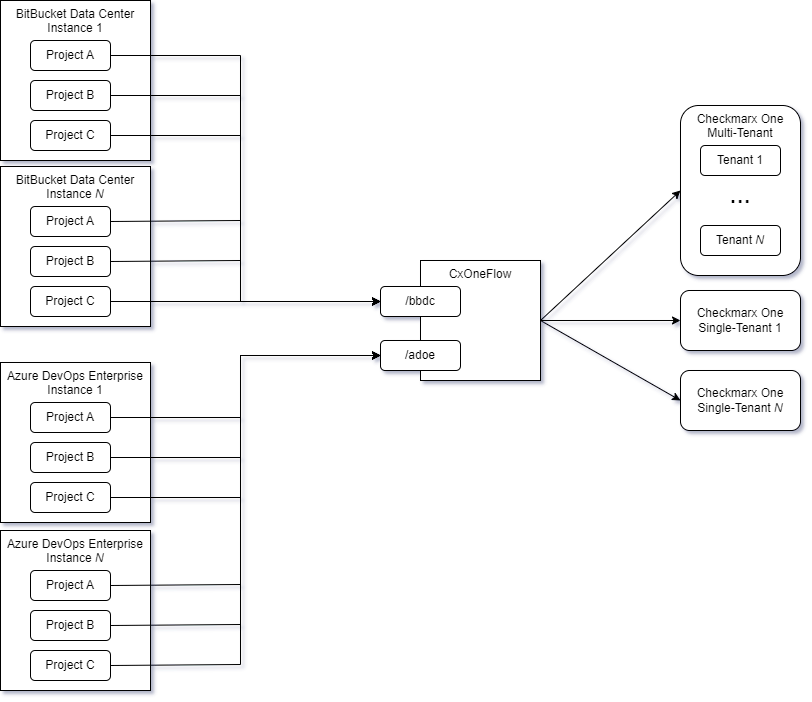
\includegraphics[width=\textwidth]{graphics/cxoneflow-deployment.png}
    \caption{\cxoneflow Deployment Diagram}
    \label{fig:cxoneflow-deployment}
\end{figure}


\chapter{Quickstart}

To get up and running with a basic configuration of \cxoneflow, these are the following steps:


\section{Step 1: Create a basic configuration YAML file}

The full configuration documentation can be found in Section \ref{sec:op-config}. To fully configure the \cxoneflow you'll need
the following information that will be used when composing the configuration YAML file:

\begin{itemize}
    \item A \cxone API Key or OAuth client id + client secret.
    \item Credentials appropriate for communicating with the Git server's API.
    \item Credentials used to clone Git repositories if the clone credentials must be different than the credentials used for API access.
\end{itemize}

\noindent\\The types of credentials may vary based on how the SCM server is configured or how \cxoneflow
integrates with the SCM.

\section{Step 2: Execute the \cxoneflow Container}

The published \cxoneflow container can be executed with the proper runtime configuration.  Please refer
to Section \ref{sec:runtime-config} for instructions about starting the \cxoneflow container instance with
the proper runtime configuration. Section \ref{sec:deployment} has additional deployment information that
may be useful in choosing how and where to host the \cxoneflow instance.


\section{Step 3: Configure SCM Webhooks}

Please refer to the chapter for your SCM platform in Part \ref{part:scms} for details about webhook configuration.



\chapter{Configuration}


\section{Runtime Configuration}\label{sec:runtime-config}

\subsection{SSL}

\subsubsection{Trusting Self-Signed Certificates}\label{sec:self-signed-certs}

While the CheckmarxOne system uses TLS certificates signed by a public CA, it is possible that
corporate proxies use certificates signed by a private CA. If so, it is possible to
import custom CA certificates when using \cxoneflow.

\noindent\\The custom certificates must meet the following criteria:

\begin{itemize}
    \item Must be in the PEM format.
    \item Must be in a file ending with the extension .crt.
    \item Only one certificate is in the file.
    \item Must be mapped to the container path /usr/local/share/ca-certificates.
\end{itemize}


\noindent\\As an example, if using Docker, it is possible to map a local file to a file in the container with this mapping option added to the container execution command line:

\begin{code}{Custom CA Mapping Option}{[Docker]}{}
-v $(pwd)/custom-ca.pem:/usr/local/share/ca-certificates/custom-ca.crt
\end{code}

\subsubsection{Configuring SSL for the \cxoneflow Endpoint}

To make the \cxoneflow endpoint use SSL for communication, obtain an SSL certificate public/private key pair
and then set the following environment variables in the runtime environment:

\begin{table}[h]
    \caption{SSL Environment Variables}        
    \begin{tabularx}{\textwidth}{ll}
        \toprule
        \textbf{Variable} & \textbf{Description}\\
        \midrule
        \texttt{SSL\_CERT\_PATH} & \makecell[l]{The path to the server's SSL certificate in PEM format.}\\
        \midrule
        \texttt{SSL\_CERT\_KEY\_PATH} & \makecell[l]{The path to the certificate's unencrypted private key.}\\
        \bottomrule
    \end{tabularx}
\end{table}

\noindent\\If your SSL certificate is self-signed or signed with a non-public CA, you'll want
to import the custom CA as described in Section \ref{sec:self-signed-certs}.


\subsection{Rutime Control Environment Variables}

\begin{table}[h]
    \caption{Runtime Control Environment Variables}        
    \begin{tabularx}{\textwidth}{lccl}
        \toprule
        \textbf{Variable} & \textbf{Required} & \textbf{Default} & \textbf{Description}\\
        \midrule
        \texttt{CXONEFLOW\_WORKERS} & No & \texttt{(\# of CPUs / 2)} & \makecell[l]{The number of worker processes\\used for parallel execution. The\\maximum value will be\\set at \texttt{(\# of CPUs - 1)}}\\
        \midrule
        \texttt{LOG\_LEVEL} & No & \texttt{INFO} & \makecell[l]{The logging verbosity level.  Set to\\\texttt{DEBUG} for increased logging\\verbosity.}\\
        \midrule
        \texttt{CONFIG\_YAML\_PATH} & No & \texttt{/opt/cxone/config.yaml} & \makecell[l]{The path to the configuration\\YAML file.}\\
        \midrule
        \texttt{CXONEFLOW\_HOSTNAME} & No & \texttt{localhost} & \makecell[l]{The virtual hostname of the\\\cxoneflow endpoint.}\\
        \bottomrule
    \end{tabularx}
\end{table}


\newpage

\section{Operational Configuration}\label{sec:op-config}

The operational configuration is done using a YAML file mapped at \texttt{/opt/cxone/config.yaml}
by default.  

\subsection{YAML Configuration Examples}

\subsubsection{Basic YAML Configurations}

The following example shows a minimal \cxoneflow configuration that defines the following:

\begin{enumerate}
    \item Files containing secrets are located at \texttt{/run/secrets}.
    \item One BitBucket Data Center SCM connection configuration to handle all webhook payloads
    POSTed to the \texttt{/bbdc} endpoint.
    \item One catch-all route for clone-urls using the regular expression \texttt{.*}
    \item The SCM's base URL located at \texttt{https://scm.corp.com}
    \item The shared secret used to validate webhook payloads located in the file \texttt{/run/secrets/scm-shared-secret}
    \item The API and clone authorization using a PAT in a file located at \texttt{/run/secrets/scm-token-secret}
    \item The CheckmarxOne tenant name of \texttt{mytenant}
    \item The CheckmarxOne API credentials using an \texttt{oauth} client with:
    \begin{enumerate}
        \item The client identifier located in the file \texttt{/run/secrets/my-oauth-id}
        \item The client secret located in the file \texttt{/run/secrets/my-oauth-secret}
    \end{enumerate}
    \item Using the CheckmarxOne multi-tenant US region IAM endpoint.
    \item Using the CheckmarxOne multi-tenant US region API endpoint.
\end{enumerate}

\begin{code}{Minimal YAML Configuration Example \#1}{[CxOne: oauth]}{[SCM: token auth]}
secret-root-path: /run/secrets

bbdc:
    - service-name: BitBucket DC
      repo-match: .*
      connection:
        base-url: https://scm.corp.com
        shared-secret: scm-shared-secret
        api-auth:
            token: scm-token-secret
      cxone:
        tenant: mytenant
        oauth:
            client-id: my-oauth-id
            client-secret: my-oauth-secret
        iam-endpoint: US
        api-endpoint: US
\end{code}

\pagebreak
\noindent\\An alternate minimal example using different authorization options:

\begin{code}{Minimal YAML Configuration Example \#2}{[CxOne: api-key]}{[SCM: basic/ssh auth]}
secret-root-path: /run/secrets

bbdc:
    - service-name: BitBucket DC
      repo-match: .*
      connection:
      base-url: https://scm.corp.com
      shared-secret: scm-shared-secret
      api-auth:
          username: scm-username-secret
          password: scm-password-secret
      clone-auth:
          ssh: scm-ssh-key-secret
      cxone:
        tenant: mytenant
        api-key: my-cxone-api-key
        iam-endpoint: US
        api-endpoint: US
\end{code}
    
\pagebreak
\noindent\\An alternate minimal example using for an Azure DevOps Enterprise
SCM:

\begin{code}{Minimal YAML Configuration Example \#2}{[CxOne: api-key]}{[SCM: basic/ssh auth]}
secret-root-path: /run/secrets

adoe:
    - service-name: MyADO
      repo-match: .*
      connection:
      base-url: https://scm.corp.com
      shared-secret: scm-shared-secret
      api-auth:
          username: scm-username-secret
          password: scm-password-secret
      clone-auth:
          ssh: scm-ssh-key-secret
      cxone:
        tenant: mytenant
        api-key: my-cxone-api-key
        iam-endpoint: US
        api-endpoint: US
\end{code}


\newpage
\noindent\\This example shows a \cxoneflow configuration explicitly setting default options in a service 
configuration for a single SCM.  The minimal examples leave several of these options as default.

The \texttt{scan-config} element has been added to this configuration to
demonstrate some of the controls that can be implemented over scan options.  In this
example, static Project and Scan tags are defined.  Also defined is the selection
of engines for the scan with some options defined as supported by the engine.
Documentation for the option keys can be found in the Checkmarx
\extlink{https://checkmarx.stoplight.io/docs/checkmarx-one-api-reference-guide/branches/main/f601dd9456e80-run-a-scan}{Scan REST API}
documentation and have the descriptions documented in the
\extlink{https://docs.checkmarx.com/en/34965-324311-settings-for-specific-scanners.html}{Scanners Settings}
documentation.

While there are options to apply scan configurations via \texttt{scan-config} elements, it is often the case that defining the scan configuration
in \cxoneflow will have undesirable results.  When defined in the \cxoneflow configuration, the configuration will explicitly override \cxone
tenant and project level default scan configurations.  Details about utilizing the \cxone configuration options for best results with \cxoneflow
can be found in Section \ref{sec:deployment-scan-defaults}.

\begin{code}{Full YAML Configuration Example}{[CxOne: oauth]}{[SCM: token auth]}
secret-root-path: /run/secrets
server-base-url: https://cxoneflow.mydomain.com:8443/

bbdc:
    - service-name: BitBucket DC
      repo-match: .*
      scan-config:
          default-scan-engines:
              sca:
                  exploitablePath: "True"
              sast:
                  presetName: ASA Premium
                  incremental: "False"
                  fastScanMode: "True"
                  filter: "!**/node_modules,!**/test*"
                  languageMode: multi
              kics:
              apisec:
          default-scan-tags:
              scan-service: BitBucket DC
          default-project-tags:
              onboarded-by: CxOneFlow
      connection:
          base-url: https://scm.corp.com
          shared-secret: scm-shared-secret
          timeout-seconds: 60
          retries: 3
          proxies:
            http: http://proxy.corp.com:8080
            https: http://proxy.corp.com:8080
          api-auth:
              token: scm-token-secret
      cxone:
          tenant: mytenant
          oauth:
              client-id: my-oauth-id
              client-secret: my-oauth-secret
          iam-endpoint: US
          api-endpoint: US
          timeout-seconds: 60
          retries: 3
          proxies:
            http: http://proxy.corp.com:8080
            https: http://proxy.corp.com:8080
\end{code}


\pagebreak
The next example shows a configuration where \cxoneflow has endpoint handlers for both
BitBucket Data Center and Azure DevOps Enterprise.  Each SCM is configured to handle multiple distinct
projects to demonstrate the use of multiple authentication methods.  All the SCM endpoints
orchestrate scans in a single \cxone tenant.

\begin{code}{Multi-SCM/Multi-Org YAML Configuration Example}{}{}
secret-root-path: /run/secrets
server-base-url: https://cxoneflow.mydomain.com:8443/
adoe-connection: &adoe-con
    base-url: http://adoe.scm.org/
    shared-secret: scm-shared-secret
bbdc-connection: &bbdc-con
    base-url: http://bbdc.scm.org
    shared-secret: scm-shared-secret
adoe:
    - service-name: ADO-EastCoast
        repo-match: .*East
        connection:
        <<: *adoe-con
        api-auth: 
            token: adoe-token-secret
        clone-auth: &clone-ssh
            ssh: ssh-priv-key
        cxone: &cxone
        tenant: my_tenant
        oauth:
            client-id: prod_client_id
            client-secret: prod_client_secret
        iam-endpoint: US
        api-endpoint: US
    - service-name: ADO-WestCoast
        repo-match: .*West
        connection:
        <<: *adoe-con
        api-auth:
            token: adoe-token-secret
        cxone: *cxone
bbdc:
    - service-name: BBDC-EastCoast
        repo-match: .*EAS
        connection:
        <<: *bbdc-con
        api-auth: 
            token: bbdc-token
        clone-auth: *clone-ssh
        cxone: *cxone
    - service-name: BBDC-WestCoast
        repo-match: .*WES
        connection:
        <<: *bbdc-con
        api-auth:
            token: bbdc-token
        cxone: *cxone
\end{code}



\subsubsection{Complex YAML Configurations using YAML Anchors}

For complex configurations, it is possible to use 
\href{https://docs.docker.com/compose/compose-file/10-fragments/}{YAML Anchors}
to avoid repeating some section definitions.  When using YAML anchors, it may be useful
to use a \href{https://onlineyamltools.com/convert-yaml-to-json}{YAML-to-JSON} conversion tool that shows the JSON generated from the YAML
definition

\noindent\\This example demonstrates defining common connection parameters that can be applied
to all connection definitions:


\begin{code}{Compacted Full YAML Configuration Example}{[CxOne: oauth]}{[SCM: token auth]}
secret-root-path: /run/secrets

my-connection-params: &common-connection-params
    timeout-seconds: 60
    retries: 3
    ssl-verify: True
    proxies:
    http: http://proxy.corp.com:8080
    https: http://proxy.corp.com:8080


bbdc:
    - service-name: BitBucket DC
      repo-match: .*
      scan-config:
          default-scan-engines:
              sca:
                  exploitablePath: "True"
              sast:
                  presetName: ASA Premium
                  incremental: "False"
                  fastScanMode: "True"
                  filter: "!**/node_modules,!**/test*"
                  languageMode: multi
              kics:
              apisec:
          default-scan-tags:
              scan-service: BitBucket DC
          default-project-tags:
              onboarded-by: CxOneFlow
      connection:
          base-url: https://scm.corp.com
          shared-secret: scm-shared-secret
          api-auth:
              token: scm-token-secret
          <<: *common-connection-params
      cxone:
          tenant: mytenant
          oauth:
              client-id: my-oauth-id
              client-secret: my-oauth-secret
          iam-endpoint: US
          api-endpoint: US
          <<: *common-connection-params
\end{code}


\noindent\\It is common to see a scenario where there are multiple organizations
using the same SCM instance.  A single \cxoneflow instance can be configured to accept
webhook events from all repos in each organization by using the \texttt{repo-match}
regular expression.  When a webhook payload is received, the \texttt{repo-match}
regular expression is applied to the clone URI until a match is found.

\noindent\\The example YAML below is used to demonstrate how \cxoneflow could be configured
for mulitple organizations in a single SCM. In the example, YAML anchors are utilized to 
re-use the common settings for each SCM organization.  Each organization, in this case, 
exists in the same SCM server and shares the same Checkmarx One instance.

\begin{code}{SCM Multi-Org YAML Configuration Example}{[CxOne: oauth]}{[SCM: token auth]}
secret-root-path: /run/secrets

my-connection-params: &common-connection-params
    timeout-seconds: 60
    retries: 3
    ssl-verify: True
    proxies:
    http: http://proxy.corp.com:8080
    https: http://proxy.corp.com:8080

bbdc:
    - service-name: BBDC-West
      repo-match: .*west
      scan-config: 
          default-scan-engines: &common-engine-config
              sca:
                  exploitablePath: "True"
              sast:
                  presetName: ASA Premium
                  incremental: "False"
                  fastScanMode: "True"
                  filter: "!**/node_modules,!**/test*"
                  languageMode: multi
              kics:
              apisec:
          default-scan-tags:
              scan-service: BBDC-West
          default-project-tags:
              onboarded-by: CxOneFlow
              region: West
      connection:
          base-url: https://scm.corp.com
          shared-secret: scm-west-org-shared-secret
          api-auth:
              token: scm-token-secret
          <<: *common-connection-params
      cxone: &cxone-config
          tenant: mytenant
          oauth:
              client-id: my-oauth-id
              client-secret: my-oauth-secret
          iam-endpoint: US
          api-endpoint: US
          <<: *common-connection-params
    - service-name: BBDC-East
      repo-match: .*east
      scan-config: 
          default-scan-engines: *common-engine-config
          default-scan-tags:
              scan-service: BBDC-East
          default-project-tags:
              onboarded-by: CxOneFlow
              region: East
      connection:
          base-url: https://scm.corp.com
          shared-secret: scm-east-org-shared-secret
          api-auth:
              token: scm-token-secret
          <<: *common-connection-params
      cxone: *cxone-config
\end{code}



\subsection{YAML Configuration Elements}

\subsubsection{YAML Root}\label{sec:yaml-root}

The root of the YAML configuration will contain the \texttt{secret-root-path} element
and one or more unique SCM configuration monikers.  The following SCM configuration monikers
are currently supported:

\begin{itemize}
    \item \texttt{bbdc} for BitBucket Data Center hook payloads targetting the \texttt{/bbdc}
    webhook payload receiver endpoint.
\end{itemize}


\noindent\\The value for \texttt{secret-root-path} is the path to a directory that contains one
or more files containing secret values.  The names to these files are referenced elsewhere
in the YAML configuration file as described in
\hyperref[sec:scm-block-element]{YAML SCM Configuration Element}.


\subsubsection{YAML SCM Configuration Element}\label{sec:scm-block-element}

The SCM configuration element is the same for all SCM monikers. The element is a list with
one or more entries corresponding to a clone URL regular expression match.  The entry
that first matches the clone URL received in the webhook payload is used to configure
the workflow execution parameters.  Table \ref{tab:scm-section-keys} explains the SCM
configuration keys for each SCM configuration list entry.

\begin{table}[h]
    \caption{SCM Configuration YAML Element}  
    \label{tab:scm-section-keys}      
    \begin{tabularx}{\textwidth}{lcl}
        \toprule
        \textbf{Key} & \textbf{Required} & \textbf{Description}\\
        \midrule
        \texttt{service-name} & Yes & \makecell[l]{A moniker for the route match that is used for logging purposes.}\\
        \midrule
        \texttt{repo-match} & Yes & \makecell[l]{A regex applied to the source repository.  If the webhook payload has\\a clone URL that matches the regex, this configuration is used to\\orchestrate the scanning.}\\
        \midrule
        \texttt{scan-config} & No & \makecell[l]{Elements that define the default scan configuration.  This element\\is described in the section\\"\hyperref[sec:scan-config-element]{YAML Configuration Element: \texttt{scan-config}}"}\\
        \midrule
        \texttt{connection} & Yes & \makecell[l]{SCM connection parameters. This element\\is described in the section\\"\hyperref[sec:connection-element]{YAML Configuration Element: \texttt{connection}}"}\\
        \midrule
        \texttt{cxone} & Yes & \makecell[l]{The connection configuration for the CheckmarxOne API. This\\element is described in the section\\"\hyperref[sec:cxone-element]{YAML Configuration Element: \texttt{cxone}}"}\\
        \bottomrule
    \end{tabularx}
\end{table}


\paragraph{YAML Configuration Element: \texttt{scan-config} }\label{sec:scan-config-element}

\noindent\\\\The \texttt{scan-config} element, described in Table \ref{tab:scan-config-section-keys}, allows for default configurations to be applied to each scan.

\begin{table}[h]
    \caption{\texttt{scan-config} YAML Element}  
    \label{tab:scan-config-section-keys}      
    \begin{tabularx}{\textwidth}{lcl}
        \toprule
        \textbf{Key} & \textbf{Required} & \textbf{Description}\\
        \midrule
        \texttt{default-scan-engines} & No & \makecell[l]{A element that follows the format\\\texttt{<engine-name>:<engine config option dictionary>}\\corresponding to the configuration element of the\\\href{https://checkmarx.stoplight.io/docs/checkmarx-one-api-reference-guide/branches/main/f601dd9456e80-run-a-scan}{Checkmarx One scan API}.}\\
        \midrule
        \texttt{default-scan-tags} & No &  \makecell[l]{A dictionary of static key:value pairs that are assigned to\\each scan.}\\
        \midrule
        \texttt{default-project-tags} & No & \makecell[l]{A dictionary of static key:value pairs that are assigned\\to each project upon project creation.}\\
        \bottomrule
    \end{tabularx}
\end{table}


\paragraph{YAML Configuration Element: \texttt{cxone} }\label{sec:cxone-element}

\noindent\\\\The \texttt{cxone} element, described in Table \ref{tab:cxone-section-keys}, 
describes the CheckmarxOne API connection parameters.


\begin{table}[h]
    \caption{\texttt{cxone} YAML Element}  
    \label{tab:cxone-section-keys}      
    \begin{tabularx}{\textwidth}{lccl}
        \toprule
        \textbf{Key} & \textbf{Required} & \textbf{Default} & \textbf{Description}\\
        \midrule
        \texttt{tenant} & Yes & N/A & \makecell[l]{The name of the CheckmarxOne tenant.}\\
        \midrule
        \texttt{iam-endpoint} & Yes & N/A & \makecell[l]{This can be a fully qualified domain name of a server\\or a multi-tenant IAM endpoint moniker as described\\in Appendix \ref{sec:endpoint-monikers}.}\\
        \midrule
        \texttt{api-endpoint} & Yes & N/A & \makecell[l]{This can be a fully qualified domain name of a server\\or a multi-tenant API endpoint moniker as described\\in Appendix \ref{sec:endpoint-monikers}.}\\
        \midrule
        \texttt{timeout-seconds} & No & 60s & \makecell[l]{The number of seconds before a request for API\\results times out.}\\
        \midrule
        \texttt{retries} & No & 3 & \makecell[l]{The number of retries when the request fails.}\\
        \midrule
        \texttt{ssl-verify} & No & True & \makecell[l]{If False, server SSL certificates are not validated.}\\
        \midrule
        \texttt{proxies} & No & N/A & \makecell[l]{A dictionary of \texttt{<scheme>:<url>} pairs to use a proxy\\server for requests. See: \href{https://requests.readthedocs.io/en/latest/user/advanced/\#proxies}{Python "requests" proxies}.}\\
        \midrule
        \texttt{api-key} & No & N/A & \makecell[l]{If not defined, the \texttt{oauth} element must be defined.\\The value specifies a file name found under the path\\defined by \texttt{secret-root-path}.}\\
        \midrule
        \texttt{oauth} & No & N/A & \makecell[l]{If not defined, the \texttt{api-key} element must be defined.\\This contains two required elements \texttt{client-id}\\and \texttt{client-secret} where each value corresponds to\\a file name found under the path defined by\\\texttt{secret-root-path}. }\\
        \bottomrule
    \end{tabularx}
\end{table}


\pagebreak
\paragraph{YAML Configuration Element: \texttt{connection} }\label{sec:connection-element}

\noindent\\\\The \texttt{connection} element, described in Table \ref{tab:connection-section-keys}, 
describes the SCM connection parameters used for API access and cloning.


\begin{table}[h]
    \caption{\texttt{connection} YAML Element}  
    \label{tab:connection-section-keys}      
    \begin{tabularx}{\textwidth}{lccl}
        \toprule
        \textbf{Key} & \textbf{Required} & \textbf{Default} & \textbf{Description}\\
        \midrule
        \texttt{base-url} & Yes & N/A & \makecell[l]{The base url of the SCM server.}\\
        \midrule
        \texttt{shared-secret} & Yes & N/A & \makecell[l]{The shared secret configured in the SCM used to sign\\webhook payloads. The shared secret must meet the\\following minimum criteria: 20 characters long,\\contains at least 3 numbers, contains at least\\3 upper-case letters, and contains at least 2 special\\characters.}\\
        \midrule
        \texttt{timeout-seconds} & No & 60s & \makecell[l]{The number of seconds before a request for API\\results times out.}\\
        \midrule
        \texttt{retries} & No & 3 & \makecell[l]{The number of retries when the request fails.}\\
        \midrule
        \texttt{ssl-verify} & No & True & \makecell[l]{If False, server SSL certificates are not validated.}\\
        \midrule
        \texttt{proxies} & No & N/A & \makecell[l]{A dictionary of \texttt{<scheme>:<url>} pairs to use a proxy\\server for requests. See: \href{https://requests.readthedocs.io/en/latest/user/advanced/\#proxies}{Python "requests" proxies}.}\\
        \midrule
        \texttt{api-auth} & Yes & N/A & \makecell[l]{A dictionary of SCM authorization options\\for using the API.\\See: \hyperref[sec:api-auth-element]{YAML Configuration Element: \texttt{api-auth}}}\\
        \midrule
        \texttt{clone-auth} & No & \makecell[l]{\texttt{api-auth}} & \makecell[l]{Authorization options for performing clones when it\\differs from authorization for API requests.\\See: \hyperref[sec:clone-auth-element]{YAML Configuration Element: \texttt{clone-auth}}}\\
        \bottomrule
    \end{tabularx}
\end{table}

\pagebreak
\paragraph{YAML Configuration Element: \texttt{clone-auth} }\label{sec:clone-auth-element}

\noindent\\\\The \texttt{clone-auth} element is optional;  if not provided, the connection information defined
in \texttt{api-auth} will be used.  This element can contain the following key:value pair combinations:

\noindent\\\textbf{Token Authorization Elements}

\noindent\\To clone with a token, the following elements can appear under the \texttt{clone-auth}
element exclusive of other elements:

\begin{itemize}
    \item \texttt{token} - The value specifies a file name found under the path defined
    by \texttt{secret-root-path} containing a Personal Access Token (PAT).  This is required for
    token authorization.
    \item \texttt{username} - The value specifies a file name found under the path defined
    by \texttt{secret-root-path} containing a username associated with the PAT.  This is 
    optional; if not supplied, the default username of \texttt{git} is used.
\end{itemize}

\noindent\\\textbf{Basic Authorization Elements}

\noindent\\To clone with basic authorization, the following required elements can appear under the
\texttt{clone-auth} element exclusive of other elements:

\begin{itemize}
    \item \texttt{username} - The value specifies a file name found under the path defined
    by \texttt{secret-root-path} containing the username associated with the account used
    for authorization. 
    \item \texttt{password} - The value specifies a file name found under the path defined
    by \texttt{secret-root-path} containing the password associated with the account used
    for authorization. 
\end{itemize}

\noindent\\\textbf{SSH Authorization Elements}

\noindent\\To clone with SSH, the following required element can appear under the
\texttt{clone-auth} element exclusive of other elements:

\begin{itemize}
    \item \texttt{ssh} - The value specifies a file name found under the path defined
    by \texttt{secret-root-path} containing an unencrypted private SSH key.
\end{itemize}

\paragraph{YAML Configuration Element: \texttt{api-auth} }\label{sec:api-auth-element}

\noindent\\\\The \texttt{api-auth} element is required.  The authorization methods for \texttt{api-auth} 
are used to communicate with the SCM's API and can often be used for cloning repositories.  The
main difference between \texttt{api-auth} and \texttt{clone-auth} is that API access generally
does not support SSH authorization. If there is a need to clone using SSH, configure the SSH
authorization under the \texttt{clone-auth} element.  This element can contain the following
key:value pair combinations:

\noindent\\\textbf{Token Authorization Elements}

\noindent\\To access the SCM API or clone with a token, the following elements can appear under the 
\texttt{api-auth} element exclusive of other elements:

\begin{itemize}
    \item \texttt{token} - The value specifies a file name found under the path defined
    by \texttt{secret-root-path} containing a Personal Access Token (PAT).  This is required for
    token authorization.
    \item \texttt{username} - The value specifies a file name found under the path defined
    by \texttt{secret-root-path} containing a username associated with the PAT.  This is 
    optional and only used during cloning; if not supplied, the default username of \texttt{git} is used.
\end{itemize}

\noindent\\\textbf{Basic Authorization Elements}

\noindent\\To access the SCM API or clone with basic authorization, the following required elements can
appear under the \texttt{api-auth} element exclusive of other elements:

\begin{itemize}
    \item \texttt{username} - The value specifies a file name found under the path defined
    by \texttt{secret-root-path} containing the username associated with the account used
    for authorization. 
    \item \texttt{password} - The value specifies a file name found under the path defined
    by \texttt{secret-root-path} containing the password associated with the account used
    for authorization. 
\end{itemize}





\chapter{Deployment}\label{sec:deployment}

If you've created a YAML configuration (Section \ref{sec:op-config}), configured your SCM to emit webhook events
(Part \ref{part:scms}) and know your runtime configuration requirements (Section \ref{sec:runtime-config}) then
you are ready to deploy.

\section{Obtaining the Container Image}

\cxoneflow is published as a container image.  If using Docker, the latest image can be pulled and cached locally
with the following command:

\begin{code}{Caching the \cxoneflow Container Image Locally}{}{}
docker pull ghcr.io/checkmarx-ts/cxone/cxone-flow:latest
\end{code}

\noindent\\While \cxoneflow is open source, making your own modified image may be difficult to support.  All
support for \cxoneflow is provided by Checkmarx Professional Services.

\section{\cxoneflow Execution}

The following is an example of a command where \cxoneflow starts and is ready to accept webhook events:

\begin{code}{\cxoneflow Example Execution}{}{}
docker run \
    -v $(pwd)/config.yaml:/opt/cxone/config.yaml \
    -v $(pwd)/secrets:/run/secrets -p 8000:8000 --rm -it \ 
    ghcr.io/checkmarx-ts/cxone/cxone-flow:latest
\end{code}

\noindent\\This executes the container with your defined \texttt{config.yml}, mapping a local directory
containing secrets files to \texttt{/run/secrets}, and exposing port 8000 locally for receipt of 
unencrypted webhook payloads.




\section{Deployment Considerations}

\subsection{Hosting}

The \cxoneflow container is stateless, listens on port 8000 for unencrypted webhook event delivery, 
and listens on port 8443 for encrypted webhook event delivery.  It is possible to map port 80 and 443
externally to the internal container ports.  A default self-signed SSL certificate will be used
for encrypted traffic via port 8443 unless a custom SSL certificate configuration is provided.  

The number of CPU cores on the host where the container is executing may be over-allocated to other
containers or processes.  Having the container use a high number of worker processes for an over-allocated
host will degrade performance.  The operation of \cxoneflow is not computationally intense
but it does perform rapid network and disk I/O when cloning source code and communicating with
remote system APIs.

It is suggested that the \cxoneflow instances are scaled to run on different physical hosts to
ensure availability.  This will mean you'll need to place the \cxoneflow host endpoints behind 
a load balancer.  The \cxoneflow endpoint \texttt{/ping} is available for monitoring each
running instance to ensure it is alive.

\subsection{Scan Configuration Defaults}\label{sec:deployment-scan-defaults}

Scan configuration defaults can be provided at the tenant-global and project scope
in CheckmarxOne.  The \cxoneflow configuration can be configured to set configuration
defaults for each scan.  It is important to understand how the CheckmarxOne default
scan configurations work given the \cxoneflow configuration can override all other
settings based on how the tenant and project defaults are configured.

The configurations in CheckmarxOne are defined in the tenant or project scope with a
flag that allows the value to be overridden at a lower level of configuration.  A
SAST scan default preset, for example, is generally configured at the tenant scope
as "ASA Premium" with the ability to override the preset at the project scope.  The
result is that initial scans that do not define a preset at the project scope or
at the time the scan is initiated use the globally-defined preset "ASA Premium".

Configuring the SAST preset in a project's settings to something other than
the SAST preset configured at the tenant scope will change the scan preset for that project.
If the tenant scope configuration was such that the SAST preset could not be overridden, the
option for configuring the preset would not appear in the project settings.

Configuring the SAST preset as a per-scan default in \cxoneflow will override both
the tenant and project scope settings if both are set to allow override.  This is 
due to the scan scope being the lowest level configuration scope.  If a project scope
configuration was such that the SAST preset could not be overridden, then the \cxoneflow
default preset set at the time of scan will be ignored.

The configurations at the tenant, project, and scan level scopes work based on overrides.
This causes the value of a configuration to be set by the lowest level in which it is
defined. This makes it possible to utilize the \cxoneflow per-scan defaults in a few
different ways.

If there are no per-scan defaults configured in \cxoneflow, all per-scan defaults
can be configured at the tenant scope.  This gives the flexibility to override 
the tenant scoped settings at the project scope; this is usually required so that
the project can configure scan settings that are specific to the project.

If per-scan defaults are configured in \cxoneflow, project scope settings can
still be set but will be overridden by the per-scan settings by default.  It will require
configuring the project settings and disabling override to prevent \cxoneflow per-scan
configurations from replacing the project scope configurations.  This may be confusing
to users who are not fully aware of how the scan configuration overrides work.

\subsubsection{\cxoneflow Inheritance of \texttt{filter} Settings}

The configuration scopes are implemented in CheckmarxOne as overrides for all
configuration elements.  This is ideal for most elements, but not ideal for elements
such as \texttt{filter} that defines the file/folder filters in each engine.  \cxoneflow
interprets \texttt{filter} settings in each scan engine so that they are inherited
in each scope rather than overridden.

\noindent\\As an example, consider these filters defined in each scope:

\begin{itemize}
    \item Tenant Scope: "!**/test,!**/tests"
    \item Project Scope "!**/*.sql"
    \item \cxoneflow Per-Scan configuration: "!**/node\_modules"
\end{itemize}

\noindent\\After \cxoneflow applies the inheritance algorithm, the resulting file/folder filter setting at the scan scope will be:
\\\\\texttt{"!**/test,!**/tests,!**/*.sql,!**/node\_modules"}


\noindent\\From a maintenance perspective, configuring tenant-scope defaults
with override enabled (such as SAST preset) can be used to avoid configuring
per-scan defaults in \cxoneflow.  It is often desirable to also set engine-specific
file/folder exclusions at the tenant scope to avoid scanning common exclusions.  
This will likely make maintaining global settings easier in most cases given
it is common to set scan defaults at the project scope.



\part{Source Control Manager Configuration}\label{part:scms}
\chapter{Common Workflow Elements}

Each source control system will use common Git concepts such as branching
and pull-requests.  Scanning workflows are orchestrated based on these common concepts as
described in Section \ref{sec:overview}.  

Some source control systems will have uncommon capabilities that can be integrated into 
the scan workflows.  Each section in this part of the manual describes any source control 
system-specific capabilities integrated into the scanning workflow.  

This section will describe common elements for each SCM that are integrated into the
scanning workflow.

\section{Created Project Naming}

In the event a scan is executed and a matching project does not exist, a new project
is created prior to the scan.  The project naming convention follows the same automatic
naming convention that is used when importing projects into \cxone using the 
Code Repository Integration.

\section{Project Tags}

In addition to any configured default project tags, Table \ref{tab:project-tags} shows
additional tags that are assigned to a project upon creation.

\begin{table}[ht]
    \caption{Project Tags}  
    \label{tab:project-tags}      
    \begin{tabularx}{\textwidth}{ll}
        \toprule
        \textbf{Tag Name} & \textbf{Value} \\
        \midrule
        \texttt{service} & \makecell[l]{The configured service name, as described in Section \ref{sec:yaml-config}, that 
        \\handled the scan workflow based on the matching route.}\\
        \midrule
        \texttt{cxone-flow} & \makecell[l]{The version of \cxoneflow that handled the scan orchestration.}\\
        \bottomrule
    \end{tabularx}
\end{table}


\section{Push Scan Tags}

When scan workflows are initiated by a "push" (e.g. a code commit to a protected branch),
the scans are assigned the tags as described in Table \ref{tab:push-scan-tags}.  These
tags are added in addition to any configured default scan tags.

\begin{table}[ht]
    \caption{Push Scan Tags}  
    \label{tab:push-scan-tags}      
    \begin{tabularx}{\textwidth}{ll}
        \toprule
        \textbf{Tag Name} & \textbf{Value} \\
        \midrule
        \texttt{commit} & \makecell[l]{The commit hash for the push the invoked the scan.}\\
        \midrule
        \texttt{workflow} & \makecell[l]{Always set to \textbf{push}.}\\
        \midrule
        \texttt{service} & \makecell[l]{The configured service name, as described in Section \ref{sec:yaml-config}, that 
        \\handled the scan workflow based on the matching route.}\\
        \midrule
        \texttt{cxone-flow} & \makecell[l]{The version of \cxoneflow that handled the scan orchestration.}\\
        \bottomrule
    \end{tabularx}
\end{table}


\section{Pull-Request Scan Tags}

Pull-Request scan tags have several tags with names matching those assigned by Push scan tags. 
Pull-Requests may follow a workflow enforced by the source control system; the state of the
Pull-Request workflow is captured in tags to the extent possible. It is not always possible
to capture the Pull-Request state accurately given it may change during a period of time
when it is not possible to update a scan's tags.  Table \ref{tab:pr-scan-tags} lists the
tags that can be observed for scans invoked by a Pull-Request event.


\begin{table}[ht]
    \caption{Pull-Request Scan Tags}  
    \label{tab:pr-scan-tags}      
    \begin{tabularx}{\textwidth}{ll}
        \toprule
        \textbf{Tag Name} & \textbf{Value} \\
        \midrule
        \texttt{commit} & \makecell[l]{The commit hash for the push the invoked the scan.}\\
        \midrule
        \texttt{workflow} & \makecell[l]{Always set to \textbf{pull-request}.}\\
        \midrule
        \texttt{service} & \makecell[l]{The configured service name, as described in Section \ref{sec:yaml-config}, that 
        \\handled the scan workflow based on the matching route.}\\
        \midrule
        \texttt{cxone-flow} & \makecell[l]{The version of \cxoneflow that handled the scan orchestration.}\\
        \midrule
        \texttt{pr-id} & \makecell[l]{The pull-request identifier that invoked the scan.}\\
        \midrule
        \texttt{pr-target} & \makecell[l]{The branch targeted by the pull-request.}\\
        \midrule
        \texttt{pr-status} & \makecell[l]{The review status of the pull-request.}\\
        \midrule
        \texttt{pr-state} & \makecell[l]{The state of the pull-request.}\\
        \bottomrule
    \end{tabularx}
\end{table}

\chapter{BitBucket Data Center}

\section{About BitBucket Data Center}

BitBucket Data Center is often confused with BitBucket Cloud; it should be noted that
the \cxoneflow configuration for BitBucket Data Center is not compatible with BitBucket Cloud.

\noindent\\The \cxoneflow endpoint \texttt{/bbdc} is the handler for all webhook event
payloads originating from BitBucket Data Center.  


\section{Webhook Configuration}

BitBucket Data Center can assign web hooks at the Project (aka Organization) level as well as at the
repository level.  Deploying web hook configurations for an enterprise-scale SCM is generally better
at the organization level since it will apply to all repositories in the organization.  Deploying
at the repository level is mostly suitable for testing purposes only.

Figure \ref{fig:bbdc-project-config} shows the BitBucket Data Center project configuration screen.  The
project key will appear in clone URLs and can be used as part of the regular expression 
placed in the \texttt{repo-match} configuration element.  Please see Section \ref{sec:scm-block-element} 
for a description of the \texttt{repo-match} configuration element.

The project's "Webhooks" configuration can be used to configure the \cxoneflow endpoint 
\texttt{/bbdc} to receive webhook events for each repository in the organization.  

\begin{figure}[h]
    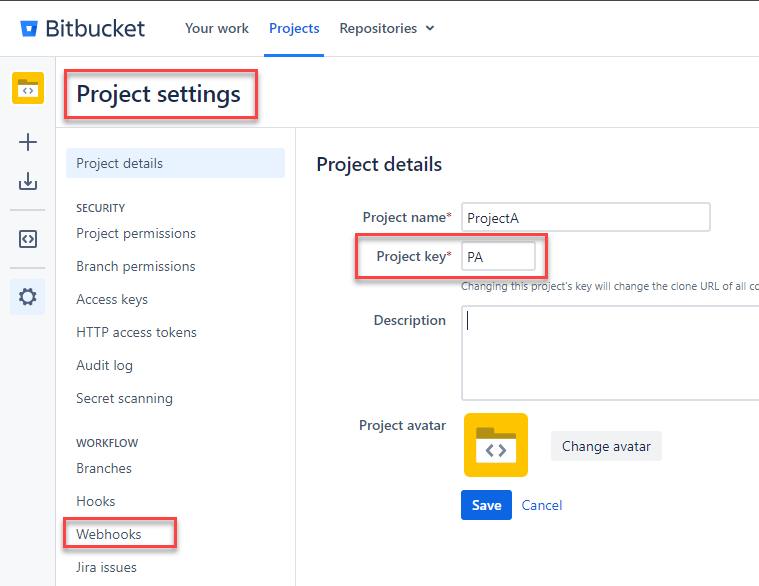
\includegraphics[width=\textwidth]{graphics/bbdc-project-config.png}
    \caption{BitBucket Data Center Project Configuration}
    \label{fig:bbdc-project-config}
\end{figure}

\begin{figure}[h]
    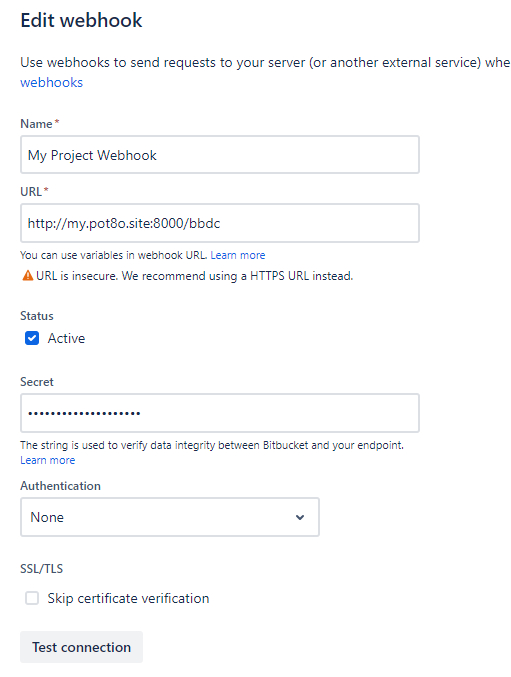
\includegraphics[width=\textwidth]{graphics/bbdc-webhook-config.png}
    \caption{BitBucket Data Center Webhook Configuration}
    \label{fig:bbdc-webhook-config}
\end{figure}



Figure \ref{fig:bbdc-webhook-config} shows a typical webhook configuration.  The Secret is how \cxoneflow
validates the origin of the event payload.  The configuration element \texttt{shared-secret}, as described
in Section \ref{sec:connection-element}, should be configured with the webhook secret value.  If \cxoneflow
is running at the specified URL endpoint, the "Test Connection" button will send a diagnostic ping
and receive back a positive response.  If the connection test fails, please ensure that \cxoneflow is running
at the address specified in the URL field and that the BitBucket Data Center server can make a connection
to that URL.

If the webhook is configured at the Project level, the events sent apply to all repositories contained
within the project.  Figure \ref{fig:bbdc-repo-event-config} shows the configured repository-level webhook 
events that will send a webhook payload to the \cxoneflow endpoint. 
Figure \ref{fig:bbdc-pr-event-config} shows the configured pull-request events that will be sent to 
the \cxoneflow endpoint.  The following events are currently supported:


\pagebreak
\begin{itemize}
    \item Repository Events
        \begin{itemize}
            \item Push
        \end{itemize}
    \item Pull Request Events
        \begin{itemize}
            \item Scanning Orchestration (Required)
                \begin{itemize}
                    \item Opened
                    \item Source branch updated
                    \item Modified
                \end{itemize}
        \end{itemize}
        \begin{itemize}
            \item Pull Request Scan Tagging (Optional)
                \begin{itemize}
                    \item Approved
                    \item Changes requested
                    \item Declined
                    \item Unapproved
                    \item Merged
                    \item Deleted
                \end{itemize}
        \end{itemize}

\end{itemize}


\begin{figure}[h]
    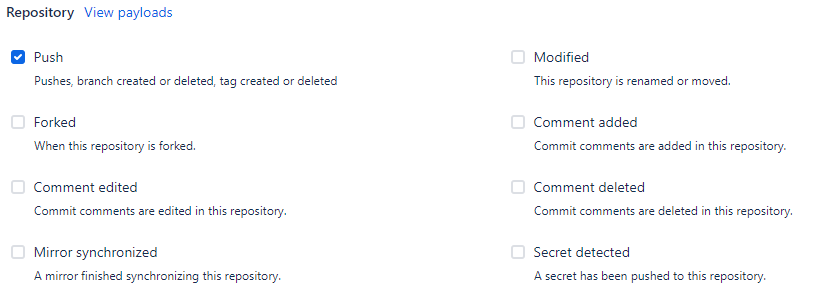
\includegraphics[width=\textwidth]{graphics/bbdc-repository-event-config.png}
    \caption{BitBucket Data Center Webhook Repository Event Config}
    \label{fig:bbdc-repo-event-config}
\end{figure}

\begin{figure}[h]
    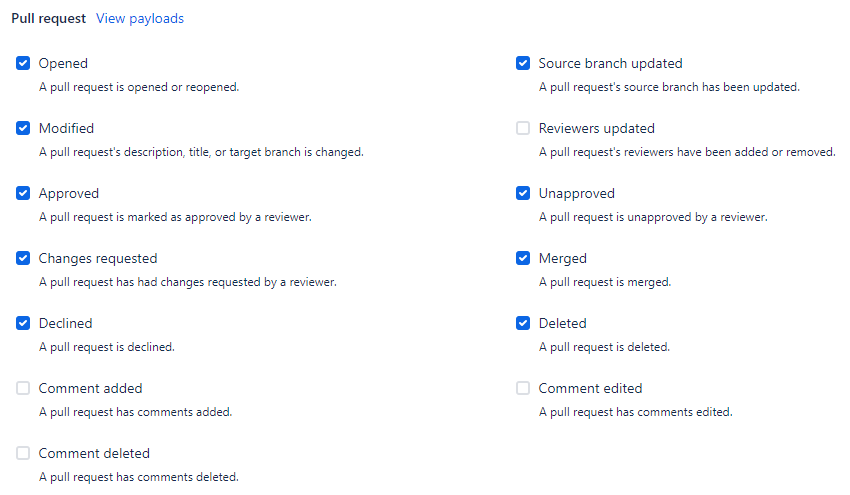
\includegraphics[width=\textwidth]{graphics/bbdc-pr-event-config.png}
    \caption{BitBucket Data Center Webhook Pull Request Event Config}
    \label{fig:bbdc-pr-event-config}
\end{figure}


\section{\cxoneflow HTTP Access Tokens}

While it is possible to use Basic Authorization to access the SCM, typically this is a configuration that
should be avoided.  The Basic Authorization is typically an interactive user account that can be subject
to password changes and Captcha verification that can break \cxoneflow operations.  It is generally
best to use a project-level HTTP Access Token for SCM connection configurations \texttt{api-auth} or
\texttt{clone-auth}.  Please refer to Section \ref{sec:connection-element} for more details about the token
configuration.

Figure \ref{fig:bbdc-token-config} shows the project-level "HTTP Access tokens" configuration.  The required
token permissions for \cxoneflow operations are:

\begin{itemize}
    \item Project read
    \item Repository read\footnote{Figure \ref{fig:bbdc-token-config} shows "Repository write".  There may be future versions of \cxoneflow that will need to create pull-request comments which will require write access.  If desired, the token can be granted "Repository read" until a write capability is released.}
\end{itemize}


\begin{figure}[h]
    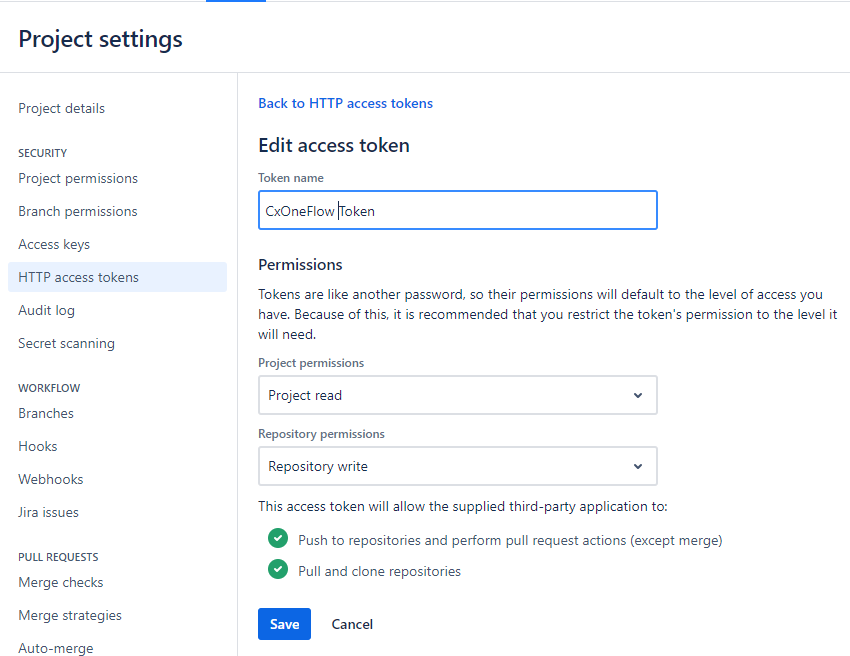
\includegraphics[width=\textwidth]{graphics/bbdc-token-config.png}
    \caption{BitBucket Data Center Project-Level HTTP Access Token Config}
    \label{fig:bbdc-token-config}
\end{figure}

Project-level access tokens do not have an associated user account.  If using project-level
access tokens, one project-level token is required per-project for which \cxoneflow is
orchestrating scans.

\section{\cxoneflow SSH Keys}

While performing scan orchestration, \cxoneflow does access the BitBucket Data Center API for
certain operations.  This requires a configuration in the \texttt{api-auth} configuration
element as described in Section \ref{sec:api-auth-element}.  The \texttt{clone-auth},
described in Section \ref{sec:clone-auth-element}, is an optional element where the credentials
used for cloning code can be provided.  If \texttt{clone-auth} is not provided, cloning will
be attempted using the credentials defined by \texttt{api-auth}.

The \texttt{clone-auth} configuration can define an SSH private key for use in cloning.  This
will allow for a separate set of credentials or authentication methods between cloning and
API use.


\section{Protected Branches}

The \cxoneflow workflow, as described in Section \ref{sec:overview}, uses the concept of "Protected Branches"
to know when to invoke workflows.  BitBucket Data Center allows for the configuration of the branching model
at the project and repository level.  Some repositories inherit their branching model from the project
configuration, but the ability for this to be overridden at the repository level is an optional configuration.
The branching model is used to determine which branches are "Protected Branches".

The project-level branching model configuration is shown in Figure \ref{fig:bbdc-branch-config}.  The
repository-level branching model configuration is similar in that both allow the definition of
"Development" and "Production" branches.  \cxoneflow considers any branch specified as a Development
or Production branch to be a "Protected Branch".

\begin{figure}[h]
    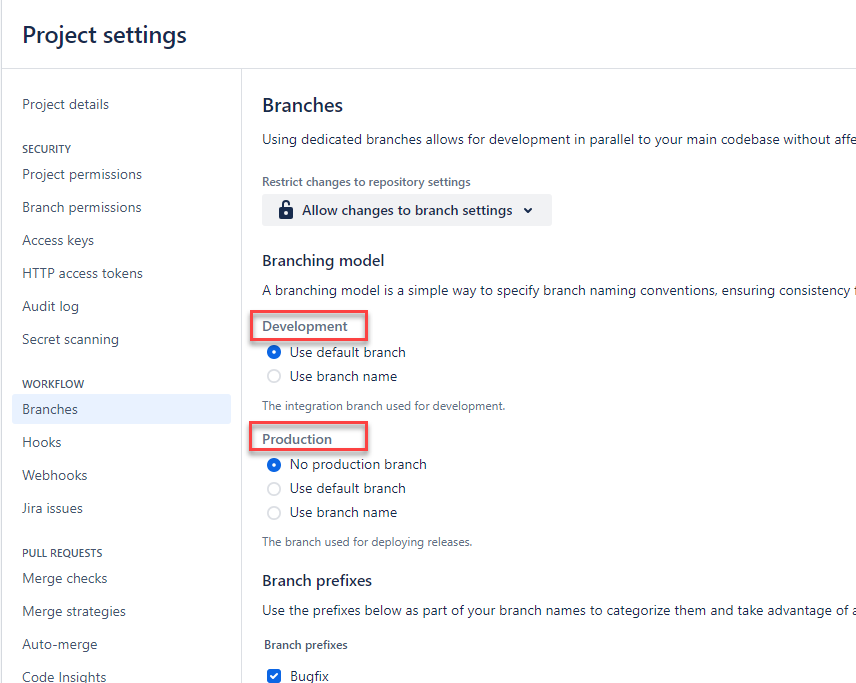
\includegraphics[width=\textwidth]{graphics/bbdc-branch-config.png}
    \caption{BitBucket Data Center Project-Level Branch Config}
    \label{fig:bbdc-branch-config}
\end{figure}


Azure DevOps Enterprise (on-premise) uses one or more \textbf{Collection} logical units to separate
repositories into logical groups.  A \textbf{Collection} in Azure DevOps Enterprise 
corresponds to a Azure DevOps Cloud \textbf{Organization} in that the \textbf{Organization} is a logical unit 
that separates repositories into logical groups. Web hook deployments are not available at this scope.

In each \textbf{Collection} or \textbf{Organization}, zero or more \textbf{Project} logical
units establish the next level of repository organization.  Each \textbf{Project} will 
have one or more \textbf{Repository} units that will contain code that should be scanned.  Webhooks
can be deployed at this scope; each \textbf{Repository} in the configured \textbf{Project} logical unit
will emit webhook events when Service Hooks have been configured in the \textbf{Project} to
deliver webhook events to \cxoneflow.

Configuration of Service Hooks at the \textbf{Project} scope is generally the preferred
method of webhook deployment for Azure DevOps.

Webhooks can be deployed at the scope of each \textbf{Repository} if desired.  The number of repositories
in a large enterprise generally makes deployment at the \textbf{Repository} scope useful
only for testing purposes.


\part{Feedback Workflows}\label{part:feedback-workflows}
\chapter{Distributed Resolver Agents}\label{sec:resolver-agents}

\section{Overview}

Executing Software Composition Analysis (SCA) scans in \cxone will gather results
by analyzing packages found in the dependency tree for the code submitted for scan.  
The \cxone SCA scan first obtains a dependency tree, then performs an analysis
of the packages found in the dependency tree. The dependency
tree is obtained by executing the same build tools normally used to develop and produce a
distributable software package.  This execution is performed using two methods: server-side 
dependency tree resolution and client-side dependency tree resolution with \scaresolver.

The purpose of the distributed resolver agent configuration with \cxoneflow is to execute a
client-side dependency tree resolution in response to a source control event.  The \cxone
\intlink{sec:overview}{scan workflow} introduces the concept of a deferred scan which delegates
a scan with \scaresolver to an appropriate distributed resolver agent instance.  The selection of
the distributed resolver agent instance is performed through a tag configuration.

The basic workflow used by \cxoneflow with distributed resolver agents is as follows:

\begin{enumerate}
  \item The SCM event is received by \cxoneflow.  If the event \intlink{sec:overview}{qualifies to invoke} a scan and
    the \intlink{sec:resolver-elements}{resolver elements} in the \cxoneflow configuration exist, \cxoneflow attempts to select
    a distributed resolver agent tag. 
  \item The \cxone project is checked for a tag matching the configured \intlink{sec:yaml-resolver-resolver-tag-key}{resolver-tag-key}.
    If the project has a tag with the matching key and the value matches one of the values in the \intlink{sec:yaml-resolver-allowed-agent-tags}{allowed-agent-tags}
    configuration, that value is selected as the distributed resolver agent's tag.
  \item If the \cxone project does not have a tag with the matching \intlink{sec:yaml-resolver-resolver-tag-key}{resolver-tag-key} and
    \intlink{sec:yaml-resolver-default-agent-tag}{default-agent-tag} is configured, the default tag is selected as the the distributed resolver agent's tag.
  \item If a distributed resolver agent tag is selected, a request for a resolver scan is sent to distributed resolver agents having the selected tag.  The
    \cxone scan is deferred until the distributed resolver agent finishes a scan.
  \item Upon notification that a distributed resolver agent has finished the resolver scan, a \cxone scan is invoked.  A tag is added to the scan
    with the key value configured in the \intlink{sec:yaml-resolver-resolver-tag-key}{resolver-tag-key} element that indicates \textbf{success} or
    \textbf{failure} of the distributed resolver agent scan.
\end{enumerate}


\subsection{Server-Side Dependency Tree Resolution}

The dependency analysis for the code submitted to \cxone is performed
in the server-side \cxone environment by executing the package managers that match the composition of the code
under scan.  This generally works sufficiently when the code references only publicly-available, open-source
packages and is compatible with the package manager tooling installed in the \cxone environment.  

Not all software is composed of only publicly available packages nor does it always use package manager tooling
that is compatible with those installed in the \cxone environment.  Incompatibilities usually manifest
when some of the following issues are observed:

\begin{itemize}
  \item The dependency tree is incomplete when software references a private package repository.
  \item The dependency tree is incomplete when the code under scan is incompatible with the 
  package manager tools installed in the \cxone environment.
\end{itemize}

If the server-side dependency resolution is not producing accurate results, the general solution is to
perform a client-side dependency tree resolution with \scaresolver. 

\subsection{Client-Side Dependency Tree Resolution with \scaresolvertext}

The \scaresolver is typically scripted to execute in
a pipeline prior to the scan submission to \cxone.  This performs the dependency resolution
in the same environment as the code builds, which will generally resolve any tooling compatibility or network connection
problems.  

Since \cxoneflow is primarily driven by asynchronous web hook events and does not invoke a pipeline
where dependency resolution can be scripted, the distributed resolver agents can perform the dependency resolution using
\scaresolver. The diagram in Figure \ref{fig:resolver-agent-diagram} shows a typical deployment of the resolver agent.  


The resolver agent is deployed such that it can execute the same build tooling as is executed during the build
in a CI/CD pipeline. The \cxoneflow server delegates \scaresolver execution to the resolver agent to perform the dependency tree
resolution; this technique is similar to how a CI/CD pipeline delegates build script execution to a system with the correct
build environment.  The build execution is sometimes performed on a self-hosted "runner" agent or executed using a container with a specified tag. 

This execution delegation technique typically results in execution of the build tools that are appropriately
configured for the normal build.  The typical CI/CD pipeline runner will also have the correct network connection paths
needed to communicate to private package repositories.


\begin{figure}[ht]
  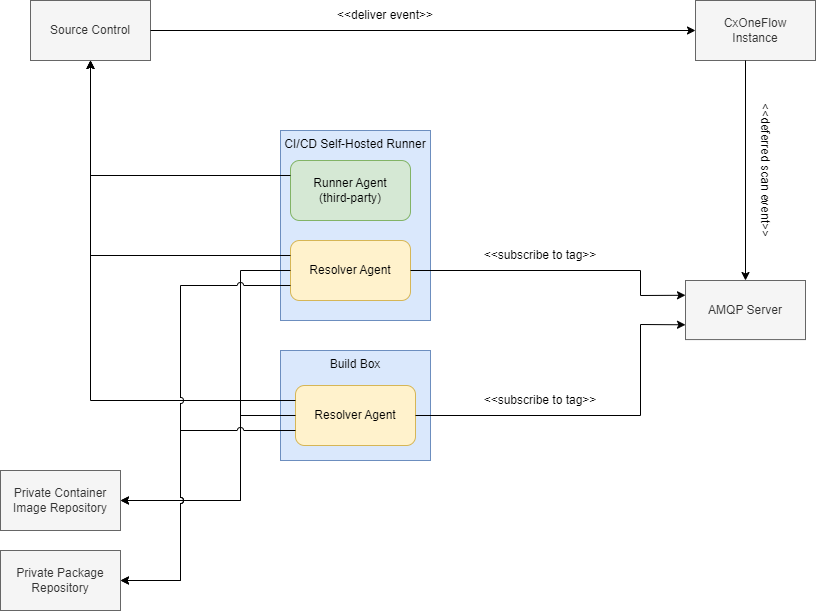
\includegraphics[width=\textwidth]{graphics/cxoneflow-diagrams-Resolver Agent Diagram.png}
  \caption{Resolver Agent Deployment Diagram}
  \label{fig:resolver-agent-diagram}
\end{figure}


\section{Distributed Resolver Security Considerations}\label{sec:dist-resolver-security-considerations}

Performing code builds, as is typically performed in a CI/CD pipeline, often includes
a bit of risk in that a build requires the execution of scripting.  There are often
controls in place to prevent anyone other than trusted authors from authoring those scripts.
As part of the scripts, there are often sensitive values exposed to the build script
for purposes of executing the build.

The use of distributed resolver agents involves some of the same risks as exist in
CI/CD pipeline builds.  To acquire a dependency tree of a project, the build tools
need to execute against the build definition to minimally produce the dependency
tree that is captured for the scan.  This action in itself can cause code to execute
as part of how the build definition is used by the tooling.  Some build tools allow
the dependencies themselves to execute code as part of the dependency resolution.
These dependencies, in some cases, can land malware in or exfiltrate data from the
environment where the dependency tree is compiled.

The \cxoneflow endpoint server itself does not invoke the build tools; this action is
delegated to the distributed resolver agents.  However, a required step of the
distributed resolver agent is to obtain a clone of the code for scanning.  To facilitate this,
the \cxoneflow endpoint server does send encoded SCM credentials to authorized
distributed resolver agents.  Section \ref{sec:resolver-agent-security} has more details
about security considerations for the distributed resolver agent.

Since the purpose of the resolver scan is to detect vulnerable and malicious packages,
it should be anticipated that malicious packages may be inadvertently referenced
by developers.  While the deployment recommendations of the distributed resolver agents
will help minimize exposure, the following security recommendations should be considered
as part of deployment of \cxoneflow with distributed resolver agents:

\begin{itemize}
  \item Use SSL for all message queue connections.
  \item Use SSL connections for delivering SCM events to the \cxoneflow endpoints.
  \item Isolate the distributed resolver agent either through installing on physically isolated machines or
  using OS permissions to isolate the distributed resolver agent runtime.
  \item Configure distributed resolver agents to execute build tools inside containers to isolate the build runtime from
  the distributed resolver agent runtime.
  \item If a scan detects a malware package, rotate all credentials used by \cxoneflow and distributed resolver agents
  after the malware is removed from the source code.
\end{itemize}

\section{Server Configuration for Distributed Resolver Agents}\label{sec:resolver-server}

Implementing the distributed resolver agents requires an AMQP message queue server that
is used for communication between the \cxoneflow server and the distributed resolver
agents.  Details about the message queue deployment can be found in Section \ref{sec:external-mq}.

\subsection{\cxoneflow Endpoint Configuration}

The endpoint server \hyperref[sec:yaml-config]{YAML configuration} will not utilize resolver agents
by default.  Using resolver agents requires a public/private key pair; the private key is configured
for use on the \cxoneflow endpoint and the public key is distributed with each resolver agent.  Before
configuring the use of distributed resolver agents, it is recommended to read about the security
concepts in Section \ref{sec:resolver-agent-security}.

The \cxoneflow endpoint will send messages signed by the private key to the distributed resolver
agents using the message queue.  The distributed resolver agents will validate the signature
using the public key; if the signature is not valid, the resolver agents will reject the message.

Distributed agents are identified using agent tags.  The \cxoneflow endpoint is configured by the
administrator with a list of allowed tags to prevent arbitrary agents from appearing.  The
server-side tag configuration is also used to set up the communication with the agents via
the message queue.  Anyone who installs a resolver agent must configure it to respond to messages
targeting at least one valid agent tag.


\subsubsection{Generating a Public/Private Key Pair}\label{ref:server-key-pair}

There are many ways to generate a public/private key pair.  There are only a few requirements
for key pairs produced by any method:

\begin{itemize}
  \item The private key must be unencrypted.
  \item Both the private and public key files must be PEM encoded.
  \item The public/private key algorithm is supported by the install Python \texttt{cryptography} library.
    As of this release, these algorithms have been tested:
  \begin{itemize}
      \item RSA 4096-bit
      \item ECDSA secp256k1
  \end{itemize}
\end{itemize}

One easy method of generating a public/private key pair is to use OpenSSL.  To generate an ECDSA public/private key pair,
the following command can be used.  The command will create the file \texttt{ec-priv.pem} that holds the unencrypted private key
and the file \texttt{ec-pub.pem} that holds the public key.

\begin{code}{OpenSSL Public/Private Key Creation}{[ECDSA]}{}
openssl ecparam -name secp256k1 -genkey -noout | tee ec-priv.pem | openssl ec -pubout > ec-pub.pem  
\end{code}

To generate an RSA 4096-bit public/private key pair,
the following command can be used.  The command will create the file \texttt{rsa-priv.pem} that holds the unencrypted private key
and the file \texttt{rsa-pub.pem} that holds the public key.

\begin{code}{OpenSSL Public/Private Key Creation}{[RSA]}{}
openssl genrsa 4096 |tee rsa-priv.pem | openssl rsa -pubout > rsa-pub.pem
\end{code}

The private key file may be stored as a secret referenced in the configuration YAML element \hyperref[sec:yaml-resolver-private-key]{resolver->private-key}.

\subsubsection{Resolver YAML Configuration}\label{sec:resolver-yaml-config}
The following YAML examples show a configuration for resolver agents with a list of allowed tags.
Some of the things to note in these examples:

\begin{itemize}
  \item The AMQP URL is stored as a secret since it contains credentials.
  \item The AMQP connection is common in both the \texttt{feedback} and \texttt{resolver} configuration.  This
  means the feedback workflows are using the same external message queue as the resolver.
\end{itemize}


\begin{code}{Minimal Resolver YAML Configuration Example}{[BitBucket Data Center]}{}
  secret-root-path: /run/secrets
  server-base-url: https://cxoneflow.mydomain.com:8443/

  amqp: &all-amqp
    amqp-url: amqp-server-credentials-secret

  bbdc:
      - service-name: BB
        repo-match: ^http(s)?:(\/){2}bitbucket\.corp\.com.*
        resolver:
          <<: *all-amqp
          private-key: resolver-agent-private-ec-key
          allowed-agent-tags:
            - thundercats
            - care-bears
            - galaxy-rangers
        feedback:
          <<: *all-amqp
          pull-request:
            enabled: True
        connection:
          base-url: https://bitbucket.corp.com
          shared-secret: scm-shared-secret
          api-auth:
            token: scm-token-secret
        cxone:
          tenant: mytenant
          oauth:
            client-id: my-oauth-id
            client-secret: my-oauth-secret
          iam-endpoint: US
          api-endpoint: US
\end{code}
  


\begin{code}{Minimal Resolver YAML Configuration Example}{[GitHub Enterprise]}{}
  secret-root-path: /run/secrets
  server-base-url: https://cxoneflow.mydomain.com:8443/

  amqp: &all-amqp
    amqp-url: amqp-server-credentials-secret

  gh:
      - service-name: GHE
        repo-match: ^http(s)?:(\/){2}github\.corp\.com.*
        resolver:
          <<: *all-amqp
          private-key: resolver-agent-private-ec-key
          allowed-agent-tags:
            - thundercats
            - care-bears
            - galaxy-rangers
        feedback:
          <<: *all-amqp
          pull-request:
            enabled: True
        connection:
          base-url: https://github.corp.com
          api-url-suffix: api/v3
          shared-secret: scm-shared-secret
          api-auth:
            app-private-key: ghc-app-priv-key
        cxone:
          tenant: mytenant
          oauth:
            client-id: my-oauth-id
            client-secret: my-oauth-secret
          iam-endpoint: US
          api-endpoint: US
\end{code}


\begin{code}{Minimal Resolver YAML Configuration Example}{[Azure DevOps]}{}
  secret-root-path: /run/secrets
  server-base-url: https://cxoneflow.mydomain.com:8443/

  amqp: &all-amqp
    amqp-url: amqp-server-credentials-secret

  adoe:
      - service-name: ADOE
        repo-match: ^http(s)?:(\/){2}ado\.corp\.com.*
        resolver:
          <<: *all-amqp
          private-key: resolver-agent-private-ec-key
          allowed-agent-tags:
            - thundercats
            - care-bears
            - galaxy-rangers
      feedback:
          <<: *all-amqp
          pull-request:
            enabled: True
        connection:
          base-url: https://ado.corp.com
          shared-secret: scm-shared-secret
          api-auth:
            token: scm-token-secret
        cxone:
          tenant: mytenant
          oauth:
            client-id: my-oauth-id
            client-secret: my-oauth-secret
          iam-endpoint: US
          api-endpoint: US
\end{code}


\subsection{Message Queue Configuration}

The \cxoneflow endpoint will configure the AMQP Exchanges and Queues upon start.  Adding any
allowed agent tags will require at least one \cxoneflow endpoint restart so that the
appropriate message queue elements for that tag can be constructed.

The message queue connection credentials for the \cxoneflow endpoint will have the 
permissions required to enable configuring the message queue elements.  Section \ref{sec:external-mq}
will give more details about the appropriate message queue user permissions for the \cxoneflow endpoint.

Configuring a distributed resolver agent will require each agent to have credentials that allow limited
access to the message queue.  Section \ref{sec:resolver-agent-security} has more details about the
authorization that should be assigned to credentials used by distributed agents.

The YAML examples in \hyperref[sec:resolver-yaml-config]{the previous section} demonstrated the use of a single
message queue instance for both the communication with the distributed resolver agents and feedback workflow
orchestration.  While using a single message queue may make the \cxoneflow configuration simpler, it is not
strictly required to use the same message queue connection for all configurations.  Each configuration can
use a segregated message queue server if this is desired.  This segregation includes the use
of \href{https://www.rabbitmq.com/docs/vhosts}{virtual hosts} if supported by the AMQP endpoint server.


\subsection{Deployment Considerations}

The YAML examples in \hyperref[sec:resolver-yaml-config]{the previous section} demonstrated agent tags
configured in a single endpoint service definition.  The allowed tags in each service endpoint are
indicating which agent tags can perform resolver scans for an event handled by that service endpoint.
The tags are used to communicate with agents that listen for messages directed to that agent tag and
have the public key associated with the private key defined in the service configuration.

The important thing to note is that distributed resolver agents are not tied to a single
\cxoneflow endpoint service definition.  The distributed resolver agents will typically have
tooling and configuration that can be used for any code that requires that tooling.  This
has some implications in how distributed resolver agents can be deployed:

\begin{itemize}
  \item The agent tag/private key pair can be different in each service definition.  It is recommended to
  use duplicate agent tags across service definitions only when those tags all share the same public/private
  key pair.

  \item Not all service definitions need to support the same allowed agent tags.  If there are distributed agents
  that should only be used by a specific service definition, it is recommended to use the allowed agent tag list
  in combination with distributed resolver connection credentials that limit the agent's ability to receive
  communications for specific tags.

  \item For complex \cxoneflow configurations that have many service definitions, it is recommended to engineer
  deployment of distributed resolver agents to be as simple as possible.
    
\end{itemize}



\section{Resolver Scan Agent Configuration}\label{sec:resolver-agent}

\subsection{Overview}


\subsection{Security Considerations}\label{sec:resolver-agent-security}

As briefly described in Section \ref{sec:dist-resolver-security-considerations}, executing
part of a code build to extract a dependency tree can pose some risks. For example,
tools like Gradle define the build definition in the programming language Groovy; this Groovy
code executes when Gradle loads the build definition.  Other tools even execute scripts defined
in the dependency package leading to the popular method of "typo-squatting" as a means to
perform a remote-code-execution (RCE) attack directly on unsuspecting developers.  Executing an
untrusted build definition or loading a dependency containing malware into a build system is
not desirable.

Since the risk of malicious builds is always possible, the deployment of the distributed resolver agent
can be configured to mitigate these risks.  The section for each platform's install makes specific
recommendations for a secure deployment of the distributed resolver agent.  The general recommendations
for all platform deployments are:

\begin{itemize}
  \item Utilize file permissions on the secret values used by the agent to limit which running processes
    can read the contents of the secrets
  \item Use the recommended directory permissions for each platform's deployment.
  \item Find a logical grouping of agents and use different message queue credentials to better avoid
    impact if any credentials are misused.
  \item Use the account security settings to limit message queue access to agents such that they are only
    able to receive and send events required for their specific operations.
  \item If the agent is invoking \scaresolver as a shell execution, utilize a "run-as" configuration to
    run the resolver as a low-privilege account.
  \item Utilize the \scaresolver docker execution capability to sandbox the dependency resolution in a container.
  \item If configuring an agent to execute \scaresolver for both shell and container dependency resolution,
    configure your docker daemon to run in "rootless" mode.
\end{itemize}


\subsubsection{Message Queue Authorization}

securing tokens/MQ creds in resolver agent


\subsubsection{Shell Agent Isolation}

securing runtime activities of the resolver agent

\paragraph{Linux}

\paragraph{Windows}
\noindent\\Distributed resolver agents are not currently supported on Windows.


\subsubsection{Container Agent Isolation}

securing runtime activities of the resolver agent

\paragraph{Linux}

\paragraph{Windows}
\noindent\\Using container agents are not supported on Windows.


\subsection{Installation}
pre-requisites:
installer for platform
message queue credentials and connection information
a public key that matches the private key deployed on the endpoint

\subsubsection{Debian Linux Platforms}

\subsection{Configuration}

\subsection{Limitations}
SSH clone does not work with resolver agent scanning


\subsection{Distributed Resolver Agent YAML Configuration}

The distributed resolver agent's YAML configuration is deployed after the agent is installed.
Many of the elements share format with the \hyperref[sec:yaml-config]{server's configuration elements}. 


Below is an example of a distributed agent YAML configuration.  This example demonstrates:

\begin{itemize}
  \item Secrets are stored in \texttt{/var/secrets}
  \item A common configuration block used by each tag is placed in each tag's configuration using YAML Anchors.
  \item \scaresolver execution uses a work path of \texttt{/var/resolver}.
  \item Shell execution of \scaresolver uses an instance installed at \texttt{/opt/resolver/ScaResolver}.
  \item Options for \scaresolver are defined in the \texttt{resolver-opts} element.
  \item All agent tags use the same AMQP configuration via YAML Anchor tags.
  \item The agent tag \texttt{general} is configured to execute \scaresolver as a shell execution.
  \item The agent tag \texttt{java-gradle} executes \scaresolver using a container image \texttt{gradle:8-jdk17-alpine} that
    is then extended by the agent using the \toolkit installed at\\\texttt{/opt/supply-chain-build-env}.
\end{itemize}


\label{code:agent-yaml-example}
\begin{code}{Distributed Resolver Agent Example Configuration YAML}{}{}
secret-root-path: /var/secrets

rabbit-cluser-amqp: &rmq-cluster
  amqp-url: amqp-cluster-url-consumer

common-config: &common
    public-key: rsa-pub.pem
    resolver-work-path: /var/resolver
    resolver-path: /opt/resolver/ScaResolver
    resolver-opts:
      log-level: Verbose
      scan-containers:
      break-on-manifest-failure:
      c: /etc/resolver/Configuration.yml
    amqp:
      <<: *rmq-cluster

serviced-tags:
  general:
    <<: *common
  java-gradle:
    <<: *common
    run-with-container:
      supply-chain-toolkit-path: /opt/supply-chain-build-env
      container-image-tag: gradle:8-jdk17-alpine
\end{code}


\pagebreak

\subsubsection{Distributed Resolver Agent YAML Configuration Tree}\label{sec:agent-yaml-root}

\dirtree{%
    .1 \hyperref[sec:agent-yaml-root]{<root>}.
    .2 \hyperref[sec:yaml-secret-root-path]{secret-root-path}\DTcomment{[Required]}.
    .2 \hyperref[sec:agent-serviced-tags]{serviced-tags}\DTcomment{[Required]}.
    .3 \hyperref[sec:agent-tag]{<agent tag>}\DTcomment{[At least 1 required]}.
    .4 \hyperref[sec:yaml-generic-amqp]{amqp}\DTcomment{[Optional] Default: localhost}.
    .5 \hyperref[sec:yaml-generic-amqp-amqp-password]{amqp-password}\DTcomment{[Optional]}.
    .5 \hyperref[sec:yaml-generic-amqp-amqp-url]{amqp-url}\DTcomment{[Required]}.
    .5 \hyperref[sec:yaml-generic-amqp-amqp-user]{amqp-user}\DTcomment{[Optional]}.
    .5 \hyperref[sec:yaml-generic-ssl-verify]{ssl-verify}\DTcomment{[Optional] Default: True}.
    .4 \hyperref[sec:agent-public-key]{public-key}\DTcomment{[Required]}.
    .4 \hyperref[sec:agent-resolver-opts]{resolver-opts}\DTcomment{[Optional] Default: None}.
    .4 \hyperref[sec:agent-resolver-path]{resolver-path}\DTcomment{[Required if not \texttt{run-with-container}]}.
    .4 \hyperref[sec:agent-resolver-run-as]{resolver-run-as}\DTcomment{[Optional] Default: run as service user}.
    .4 \hyperref[sec:agent-resolver-work-path]{resolver-work-path}\DTcomment{[Optional] Default: /tmp/resolver}.
    .4 \hyperref[sec:agent-run-with-container]{run-with-container}\DTcomment{[Required if not \texttt{resolver-path}]}.
    .5 \hyperref[sec:agent-container-image-tag]{container-image-tag}\DTcomment{[Required]}.
    .5 \hyperref[sec:agent-supply-chain-toolkit-path]{supply-chain-toolkit-path}\DTcomment{[Required]}.
    .5 \hyperref[sec:agent-use-running]{use-running-gid}\DTcomment{[Optional] Default: True}.
    .5 \hyperref[sec:agent-use-running]{use-running-uid}\DTcomment{[Optional] Default: True}.
}

\subsubsection{YAML Element: Root}\label{sec:yaml-root}

The root elements of the YAML configuration are formatted to the left-most
position in the YAML file.  Anchor elements may be defined at the root but
must not clash with the names of any of the root elements.

\subsubsection{YAML Element: secret-root-path}\label{sec:yaml-secret-root-path}

A string that is the path to a directory that contains one or more files containing secret values.  The names to these files are 
referenced elsewhere in the YAML configuration file when used in a field that is a reference to a secret.

\subsubsection{YAML Element: server-base-url}\label{sec:yaml-server-base-url}
A string that is the base URL for the \cxoneflow endpoint.  This is used when creating feedback content that loads image elements.

\subsubsection{YAML Element: <scm moniker>}\label{sec:yaml-scm-monikers}

This is a moniker indicating the a list of service definitions for handling events from an SCM matching the name of the SCM
moniker.  Each service definition is a YAML dictionary of elements. The contents for each service definition dictionary 
have the same meaning unless otherwise specified.  At lease one SCM moniker with one configured service definition is required. 
The following SCM configuration monikers are currently supported:

\begin{itemize}
    \item \textbf{\texttt{bbdc}} for BitBucket Data Center webhook payloads targeting the \texttt{/bbdc}
    webhook payload receiver endpoint.
    \item \textbf{\texttt{adoe}} for Azure DevOps Enterprise or Cloud webhook payloads targeting the \texttt{/adoe}
    webhook payload receiver endpoint.
    \item \textbf{\texttt{gh}} for GitHub Enterprise or Cloud webhook payloads targeting the \texttt{/gh}
    webhook payload receiver endpoint.
\end{itemize}


\subsubsection{<agent tag>}\label{sec:agent-tag}
A tag name that matches a value in the server-side \hyperref[sec:yaml-resolver-allowed-agent-tags]{allowed-agent-tags}
list.  The agent will listen for scan requests sent for this tag and perform the \scaresolver scan
based on the configuration for this tag.

\subsubsection{public-key}\label{sec:agent-public-key}
The value specifies a file name found under the path defined by \texttt{secret-root-path} containing a 
public key that matches the server's configured \hyperref[sec:yaml-resolver-private-key]{\texttt{private-key}} setting.

\subsubsection{resolver-opts}\label{sec:agent-resolver-opts}
This is a dictionary of
\href{https://docs.checkmarx.com/en/34965-132888-checkmarx-sca-resolver-configuration-arguments.html#UUID-bc93274b-c1c7-ea47-9556-3bd8900711dc_id_CheckmarxSCAResolverConfigurationArguments-ConfigurationArguments-TablesandSamples}{configuration arguments}
passed to \scaresolver when executing.  The options are used to provide static values for resolver execution configuration.  Some of the
options may clash with execution options provided by the agent; options that would clash with how the agent executes \scaresolver are ignored.  

The \texttt{resolver-opts} section is a dictionary of key and key/value pairs. The \hyperref[code:agent-yaml-example]{agent YAML configuration example}
shows the use of the following \scaresolver configuration parameters:

\begin{itemize}
  \item The key \texttt{log-level} with the value \texttt{Verbose} produces the configuration\\option: \texttt{--log-level=Verbose}
  \item The key \texttt{scan-containers} with no value produces the configuration\\option: \texttt{--scan-containers}
  \item The key \texttt{break-on-manifest-failure} with no value produces the configuration\\option: \texttt{--break-on-manifest-failure}
  \item The key \texttt{c} with the value \texttt{/etc/resolver/Configuration.yml} produces the configuration\\option: \texttt{-c=/etc/resolver/Configuration.yml}
\end{itemize}


These options, if set, will be ignored:

\begin{itemize}
  \item a | account
  \item containers-result-path
  \item resolver-result-path
  \item project-name
  \item authentication-server-url
  \item p | password
  \item sso-provider
  \item sca-app-url
  \item s | scan-path
  \item server-url
  \item u | username
  \item project-tags
  \item scan-tags
  \item bypass-exitcode
  \item no-upload-manifest
  \item help
  \item manifests-path
  \item t | project-teams
  \item q | quiet
  \item save-evidence-path
  \item severity-threshold
  \item report-content
  \item report-extension
  \item report-path
  \item report-type
  \item sast-result-path
  \item cxpassword
  \item cxuser
  \item cxprojectid
  \item cxprojectname
  \item cxserver
\end{itemize}

\subsubsection{resolver-path}\label{sec:agent-resolver-path}
The path to the \scaresolver executable that has been installed on the system running the distributed resolver agent.


\subsubsection{resolver-run-as}\label{sec:agent-resolver-run-as}
The name of a user account that will run the \scaresolver when executed in a shell (but not as a container).  This
is an advanced configuration that will require additional configuration for your platform.  

If not provided, the \scaresolver is executed as the same user that is running the distributed resolver agent service.

\subsubsection{resolver-work-path}\label{sec:agent-resolver-work-path}
A path where temporary files are written during the operation of the distributed resolver agent.  This also serves as the home
directory for the distributed resolver agent user and the user defined in \texttt{resolver-run-as}.


\subsubsection{run-with-container}\label{sec:agent-run-with-container}
A YAML dictionary with key/value pairs used to define running \scaresolver in a container.  If this is supplied,
the configured \texttt{resolver-path} is ignored and \scaresolver will not be invoked in a shell.  The dependency
tree collected by \scaresolver will be done by executing build tools defined in the container.  This is useful for
organizations that utilize containerized build environments in their CI/CD pipeline build scripts.

The use of containers to run \scaresolver is not supported on Windows platforms.

\subsubsection{container-image-tag}\label{sec:agent-container-image-tag}
The container tag that is found in one of the logged-in container registries.  This container tag is used by the \toolkit
to create an extended image with \scaresolver installed.

\subsubsection{supply-chain-toolkit-path}\label{sec:agent-supply-chain-toolkit-path}
The path where the \toolkit build environment is installed.

\subsubsection{use-running-gid and use-running-uid}\label{sec:agent-use-running}
These options are True by default.  This causes the image built by the \toolkit to use the
UID and primary GID of the user running the distributed resolver agent when defining a non-root
user in the extended image.  

The reason for this is that when \scaresolver is executed in the container, temporary paths
in the \texttt{resolver-work-path} are mapped to the container.  Files created by the container
will have the UID/GID of the running container's user when created.  Since the UID/GID of the
container matches the UID/GID of the distributed resolver agent, the files that remain after
the container exits can be controlled by the distributed resolver agent.

Setting these values to False should only be done in circumstances where the UID/GID for written files
should be defined by the container.  This scenario may never practically exist.








\part{Appendices}
\appendix
\chapter{Release Notes}

\let\sectionold\thesection

\renewcommand\thesection{v}

\section{1.2}

\begin{itemize}
    \item Fixed problem where pooled connections to the SCM would cause PR failures when the network routing 
    fabric discarded the connection route.
    \item BREAKING CHANGE - Added a new configuration option for the CxOneFlow server base URL used to host image
    artifacts used in PR feedback comments.
    \item Fixed an issue with \texttt{ssl-verify} not working with self-signed CAs.
    \item Documentation updates.
\end{itemize}


\section{1.1}

\begin{itemize}
    \item Added more verbose logging to aid in troubleshooting feedback workflows.
    \item Fixed an issue where the feedback scan polling parameters were ignored in some configurations.
    \item Added result summary to PR feedback comments.
    \item If detailed PR feedback comment content exceeds the SCM's comment limit, the comment will be limited to the summary content.
    \item Fixed an issue with the scan permalink published in the PR feedback comments.
\end{itemize}


\section{1.0}

\begin{itemize}
    \item Stabilize Azure DevOps Enterprise Cloud basic authorization implementation.
    \item ADO service hook test ping now fails if the correct shared secret is not provided.
\end{itemize}


\section{0.2 - Beta Release}
   

\begin{itemize}
    \item Support for Azure DevOps Enterprise Cloud.
    \item Pull-request feedback.
\end{itemize}

\section{0.1 - Initial Beta Release}
   

\begin{itemize}
    \item Support for BitBucket Data Center 8.19.2\footnote{Testing was performed against 8.19.2 but it is possible that earlier versions will work.}
    \item Support for Azure DevOps Enterprise 2022.1\footnote{Testing was performed against 2022.1 but it is possible that earlier versions will work.}
    \item Webhook Endpoint support for BitBucket Data Center (BBDC) and Azure DevOps Enterprise (ADOE).
    \item Scan on push to protected branches.
    \item Scan on pull-request targetting protected branches.
    \item Pull-request workflow scan tagging.
\end{itemize}

\let\thesection\sectionold

\chapter{Running \cxoneflowtext\space as a \texttt{systemd} Service}


Running \cxoneflow as a \texttt{systemd} service on Linux is one method that
will allow the container to be started automatically when the hosting system
is rebooted.  The \texttt{systemd} service can then be used to start and stop the
\cxoneflow services.  This section details an example configuration that can be adapted
to your environment.


\section{Obtain and Store Files}

In the directory \texttt{/opt/cxoneflow}, collect the configuration YAML, PEM encoded SSL certificate, PEM encoded SSL certificate private key,
and any secret\footnote{If planning to map secrets to the container using other methods, 
writing the files is not required.} files referenced in the configuration YAML.  The following
ownership and permissions files are suggested:

\begin{itemize}
    \item Set the ownership to \texttt{root:docker} with the command \texttt{chown -R root:docker /opt/cxoneflow}
    \item Set the permissions of \texttt{/opt/cxoneflow} using the command \texttt{chmod 750 /opt/cxoneflow}
    \item Set the permissions of the files in \texttt{/opt/cxoneflow} using the command
    \texttt{chmod -R 740 /opt/cxoneflow/*}
\end{itemize}


\section{Container Creation}

Creating a reusable container with the name \textbf{cxoneflow} can be done with the following
command:

\begin{code}{Container Creation Command}{}{}
docker create --name "cxoneflow" -p 443:8443 --env-file runtime.env \
  -v /path/to/cert.pem:/opt/cxone/certs/mycert.pem \
  -v /path/to/private.key.pem:/opt/cxone/certs/my.private.key.pem \
  -v /path/to/config.yaml:/opt/cxone/config.yaml \
  -v /path/to/secrets:/run/secrets \
  ghcr.io/checkmarx-ts/cxone/cxone-flow:latest
\end{code}

\noindent\\The command creates a container with the following properties:

\begin{itemize}
    \item The container with the name \textbf{cxoneflow} is created.
    \item Port 443 is mapped to port 8443 of the container to support secure communication with
    the \cxoneflow endpoint.
    \item Runtime environment variables (as described in Section \ref{sec:runtime-config}) 
    located in the file \texttt{runtime.env} are injected into the container's environment.
    \item Maps the following files from the local \texttt{/path/to/} path to files for the SSL
    certificate, configuration YAML, and secrets
    \footnote{This is assuming the secrets are not already mapped to the container using other methods.}.
\end{itemize}

\noindent\\It is suggested that the command is incorporated into a shell script so it may be
invoked to recreate the container during a version upgrade.

\section{Service Definition}

A \texttt{systemd} service definition should be created using a file named, for example,
\\\texttt{/opt/cxoneflow/cxoneflow.service}.  The service definition should have contents
similar to the following:

\begin{code}{/opt/cxoneflow/cxoneflow.service}{}{}
[Unit]
Description=CxOneFlow container
Requires=docker.service
After=docker.service

[Service]
Restart=always
ExecStart=/usr/bin/docker start -a cxoneflow
ExecStop=/usr/bin/docker stop cxoneflow
Type=exec

[Install]
WantedBy=default.target
        
\end{code}

\noindent\\The service definition allows \texttt{systemd} to manage the start
and stop of the \cxoneflow service in response to system startup and shutdown.


\section{Enable and Start the \cxoneflowtext Service}

The following commands will enable the service to start automatically 
on reboot and start \cxoneflow:

\begin{code}{}{}{}
sudo systemctl enable /opt/cxoneflow/cxoneflow.service
sudo systemctl start cxoneflow
\end{code}

\section{Upgrading}

A new instance of \cxoneflow can be upgraded with the following steps:

\begin{enumerate}
  \item Stop the \cxoneflow systemd service.
  \item Remove the \texttt{cxoneflow} container instance.
  \item Pull the latest \cxoneflow container image.
  \item Recreate the \texttt{cxoneflow} container image.
  \item Start the \cxoneflow systemd service.
\end{enumerate}



\begin{code}{Upgrade Commands}{}{}
  sudo systemctl stop cxoneflow
  docker container rm cxoneflow
  docker pull ghcr.io/checkmarx-ts/cxone/cxone-flow:latest
  <... docker create command ..>
  sudo systemctl start cxoneflow
\end{code}
 



\chapter{High Availability and Resolver Agent Deployments}
\label{sec:high-availability}

\section{Overview}

\cxoneflow can be deployed in a high-availability configuration using multiple instances of
the \cxoneflow container.  The \cxoneflow instances need to have a shared MQ cluster that
can communicate with the AMQP protocol.  The MQ instance is where long-running state data
is persisted by each instance.  Figure \ref{fig:ha-diagram} shows a deployment diagram for
a typical high-availability configuration.


\begin{figure}[h]
    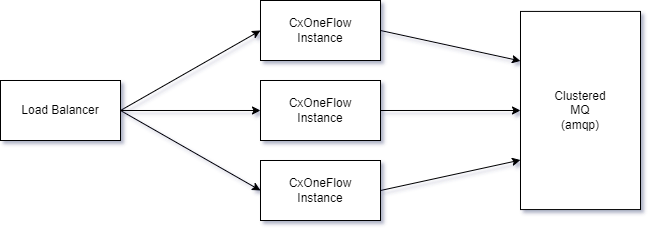
\includegraphics[width=\textwidth]{graphics/cxoneflow-diagrams-HA.png}
    \caption{High Availability Deployment Diagram}
    \label{fig:ha-diagram}
\end{figure}


\section{Load Balancing \cxoneflowtext\space Endpoints}

A typical load balancer round-robin configuration can be used to load balance \cxoneflow endpoint container instances.
There is no user interface component to \cxoneflow; this means that each connection to the \cxoneflow endpoint is stateless
and will not require any session-affinity (aka sticky-sessions) settings on the load balancer.

The \texttt{/ping} endpoint on the \cxoneflow container can be used for health-check by the load balancer.  
It is recommended that all instances of the \cxoneflow endpoint containers are using the same version.

Multiple \cxoneflow endpoint containers behind a load balancer is recommended but not technically required
when deploying \intlink{sec:resolver-agent}{resolver agents}.  However, an external message queue shared by the \cxoneflow endpoints
and the resolver agent instances is required to distribute resolver scan jobs and results.  

\section{External Message Queue}\label{sec:external-mq}

An external message queue is required for high-availability deployments of \cxoneflow or deployments that use distributed
\intlink{sec:resolver-agent}{resolver agents}.  Although a single instance of an external message queue can be used, it is
recommended that the external message queue use a clustered configuration for purposes of high-availability.  The message queue
must understand the AMQP protocol and be able to implement the concepts of Topic Exchanges, replicated queues, and queue
dead-letter exchanges.  While there may be many message queue servers that understand AMQP, the recommended message queue
server is RabbitMQ.\footnote{The "Amazon MQ Service" in AWS can be used to easily deploy a managed RabbitMQ cluster.}

It is highly recommended to create a \textbf{non-administrative} message queue user for use in the \cxoneflow endpoint
connection configuration.  The user account connected to the MQ must have the ability to configure the
exchange and queue schema.  The user permissions configuration may vary by message queue platforms; the user permissions
needed when using RabbitMQ can be found in Table \ref{tab:server-mq-user-perms}.  

Note that the permissions in Table \ref{tab:server-mq-user-perms} are not the same permissions
that should be applied in \intlink{sec:resolver-agent}{resolver agent} configurations; please see Chapter \ref{sec:resolver-agent} for more
information about message queue user permissions for resolver agents.

\begin{table}[ht]
    \caption{RabbitMQ User Permissions for the \cxoneflow Endpoint}  
    \label{tab:server-mq-user-perms}      
    \begin{tabularx}{\textwidth}{lcl}
        \toprule
        \textbf{Permission} & \textbf{Regular Expression} \\
        \midrule
        \texttt{Configure} & \texttt{\^{}cx:.*} \\
        \midrule
        \texttt{Write} & \texttt{\^{}cx:.*} \\
        \midrule
        \texttt{Read} & \texttt{\^{}cx:.*} \\
        \midrule
        \bottomrule
    \end{tabularx}
\end{table}




\chapter{\cxonetext\space Multi-Tenant Endpoint Monikers}
\label{sec:endpoint-monikers}


\section{IAM Endpoint Monikers}

These endpoint monikers correspond to the IAM endpoints referenced in the 
\extlink{https://checkmarx.stoplight.io/docs/checkmarx-one-api-reference-guide/branches/main/ywuqb5n3fas83-authentication-api\#url}{\cxonetext Authentication API} documentation.

\begin{itemize}
    \item US
    \item US2
    \item EU
    \item EU2
    \item DEU
    \item ANZ
    \item India
    \item Singapore
    \item UAE
\end{itemize}


\section{API Endpoint Monikers}

These endpoint monikers correspond to the API endpoints referenced in several
API endpoint descriptions such as the one for 
\extlink{https://checkmarx.stoplight.io/docs/checkmarx-one-api-reference-guide/branches/main/ry3bnvw1ikz2h-projects-rest-api}{\cxonetext Projects REST API} documentation.




\begin{itemize}
    \item US
    \item US2
    \item EU
    \item EU2
    \item DEU
    \item ANZ
    \item India
    \item Singapore
    \item UAE
\end{itemize}

\chapter{Troubleshooting}

If \cxoneflow does not appear to be operating as expected, the following
troubleshooting steps may help to understand the reason:

\begin{itemize}
    \item The environment variable \texttt{LOG\_LEVEL} can be set to \texttt{DEBUG}
    to emit trace information as \cxoneflow is running.

    \item Navigate to the \texttt{ping} endpoint in your browser to see the 
    \texttt{pong} response using: \texttt{http://<server>/ping}
    
    \item The \cxoneflow logs are streamed to the container's stdout.  It can be
    viewed by running the container interactively or using a command such as
    \texttt{docker logs -f <container name>}

    \item Nginx and Gunicorn logs can be found in \texttt{/var/log} on the container
    image.  A shell on the container can be opened using a command such as
    \texttt{docker exec -it <container name> bash}

    \item For Git cloning issues, the setting environment variables \texttt{GIT\_TRACE=1} and
    \texttt{GIT\_CURL\_VERBOSE=1} may log useful troubleshooting information.

\end{itemize}

\noindent\\Exception stack traces emitted in the \cxoneflow logs can generally
indicate any issues it is encountering.  Many issues are likely to be configuration
related.
\chapter{AMQP Workflow Orchestration}\label{sec:amqp-workflow-orch}



\section{Overview}

A message queue that supports the AMQP protocol is used to maintain state for \cxoneflow
workflows.  The schema for the exchanges and queues is depicted in Figure \ref{fig:amqp-schema}.
The \texttt{Scan In} exchange is the entrypoint for all workflow state messages.  It is possible
to bind custom topic exchanges and create custom queues to augment or replace some of the
workflows.


\begin{figure}[h]
    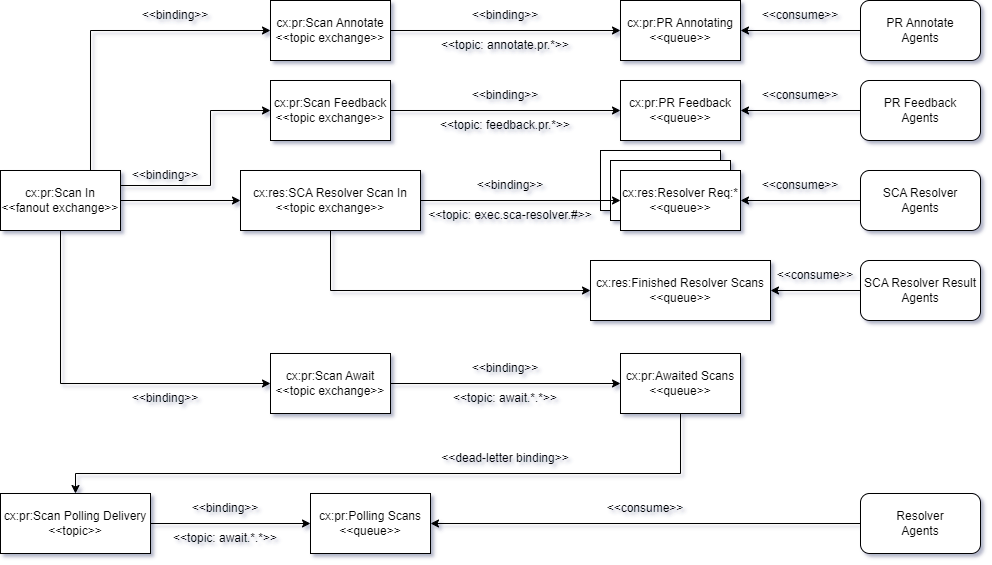
\includegraphics[width=\textwidth]{graphics/cxoneflow-diagrams-Queue.png}
    \caption{AMQP Schema for \cxoneflow}
    \label{fig:amqp-schema}
\end{figure}


\noindent\\Upon startup, each \cxoneflow instance will configure the exchange/queue schema.  An
internal instance of RabbitMQ runs inside the \cxoneflow container to orchestrate
workflows for the container instance.  If an AMQP connection configuration, described in
Section \ref{sec:amqp-element}, is not provided then the local RabbitMQ instance is
used.  When the container is exited, all persisted workflow state information in the local
RabbitMQ instance is lost.  To persist workflow state across container restarts, please
refer to Appendix \ref{sec:high-availability} to deploy \cxoneflow in a
high-availability configuration.

\section{Message Topic Format}

Messages enqueued via the \texttt{Scan In} exchange will have a topic in the format of:

\begin{code}{}{}{}
<scan state>.<workflow>.<service moniker>
\end{code}

\noindent\\Current scan states are:

\begin{itemize}
    \item await
    \item feedback
    \item annotate
\end{itemize}

\noindent\\The \texttt{Scan In} exchange is a fanout exchange that is bound to several topic
exchanges.  The topic for the message submitted to the \texttt{Scan In} exchange is used to
route the message by each bound topic exchange.

\noindent\\For customization purposes, other topic
exchanges may be bound to the \texttt{Scan In} exchange.\footnote{Integration concepts
using AMQP topic exchanges are beyond the scope of this manual.} When a \cxoneflow instance starts,
any customized bindings to the \texttt{Scan In} exchange are not modified.


\noindent\\The \texttt{moniker} segment of the topic is set to the value of the
SCM configurations \texttt{service-name} element as described in
Section \ref{sec:scm-block-element}.

\subsection{The \texttt{await} Scan State}

Messages with the scan state segment of the topic set to \texttt{await} can have the following
values in the workflow segment:

\begin{itemize}
    \item pr
    \item push
\end{itemize}

\noindent\\The \cxoneflow agents send this message when a scan is started.  This begins
the workflow that monitors the state of the scan to detect when the scan finishes
or fails before beginning the next workflow.


\subsection{The \texttt{annotate} Scan State}

Messages with the scan state segment of the topic set to \texttt{annotate} can have the following
values in the workflow segment:

\begin{itemize}
    \item pr
\end{itemize}

\noindent\\The \texttt{annotate} state is used by the workflow to note the status of the
scan.  Please refer to Part \ref{sec:feedback-workflows} for details about each supported
workflow.


\subsection{The \texttt{feedback} Scan State}

Messages with the scan state segment of the topic set to \texttt{feedback} can have the following
values in the workflow segment:

\begin{itemize}
    \item pr
\end{itemize}

\noindent\\The \texttt{feedback} state is used by the workflow to map scan result data to
a feedback method appropriate for the scan type workflow.  
Please refer to Part \ref{sec:feedback-workflows} for details about each supported workflow.

\chapter{\cxoneflowtext\space Developer Information}\label{sec:cxoneflow-development}

The development is performed on Ubuntu using Visual Studio Code.  This is not 
strictly required but any instructions for quick starting the development environment 
will be for using Ubuntu and VSCode. If you have different development tooling you'd like
to use, you'll need to adapt these instructions to fit your tooling.

The target version of Python is currently 3.12.  Using versions prior to 3.12 will likely result in
runtime errors.

\section{Secrets}

\textbf{DO NOT COMMIT SECRETS}

In general, it is a bad idea to commit secrets to the repository.  The \texttt{.gitignore} file is configured
to ignore folders named \texttt{secrets} and YAML files in the root of the code directory.  This 
can be circumvented or other files containing secrets can be inadvertently committed.

If you've committed secrets but not pushed to the public GitHub repository, you can edit the commit history
or merge your clean code into a new clone.  If you've pushed a secret into the public repository, please notify
the other maintainers so the impact can be assessed.

\section{Running with a Debugger}

The VSCode debug menu has a \texttt{Flask} debug task that will run a single endpoint locally.  By default,
the code will attempt to open \texttt{./config.yaml} for the YAML configuration.  Provide a
\texttt{config.yaml} file in the root of your development environment or set the appropriate environment
variables with the path to your \texttt{config.yaml} file.


\section{Installing \LaTeX\space for Documentation}

The documentation is written in LaTeX, so enabling VSCode to lint, compile, and preview
LaTeX requires some configuration.

\subsection{\LaTeX\space Setup}

Follow these steps to install \LaTeX.

\begin{enumerate}
    \item In VSCode, install the "LaTeX Workshop" plugin by James Yu

    \item Install TexLive direct from the website.  This is required since
    most Debian package repositories have an older version of TexLive.
    \begin{enumerate}
        \item Download instructions: \extlink{https://www.tug.org/texlive/acquire-netinstall.html}{https://www.tug.org/texlive/acquire-netinstall.html}
        \item Install instructions: \extlink{https://www.tug.org/texlive/quickinstall.html}{https://www.tug.org/texlive/quickinstall.html}
    \end{enumerate}

    \item At the end of the install, it will instruct you to update `PATH`, `MANPATH`, and `INFOPATH`.
    Set these in `~/.bashrc`, close your shell and re-open it to get the new environment variables.

    \item Execute \texttt{sudo \$(which texconfig) rehash}

\end{enumerate}

If \LaTeX\space is installed correctly, opening any of the \texttt{.tex} files will prove the ability to
compile and preview the manual PDF.



\end{document}
